% Do not change document class, margins, fonts, etc.
\documentclass[a4paper,oneside,bibliography=totoc]{scrbook}
\setlength{\parindent}{25pt}
\newtheorem{definition}{Definition} \newtheorem{proposition}{Proposition}
\usepackage{appendix}

% Add packages
\usepackage[
colorlinks=true, urlcolor=blue, linkcolor=black, colorlinks,citecolor=green
]{hyperref}
\usepackage[utf8]{inputenc}
\usepackage{emptypage}
\usepackage{enumitem}
\usepackage{graphicx}
\usepackage[justification=raggedright]{caption}
\captionsetup{labelformat=empty, textformat=empty}
\usepackage{latexsym}
\usepackage{amsmath}
\usepackage{amssymb}
\usepackage{tabularx}
\usepackage{booktabs}
\usepackage{pdflscape}
\usepackage{algorithm} % you can modify the algorithm style to your liking
\usepackage{algorithmic}
\usepackage{csquotes}
\renewcommand{\algorithmiccomment}[1]{\hfill\textit{// #1}}
\usepackage[usenames,dvipsnames]{xcolor}
\usepackage[nopostdot, style=super, nogroupskip, nonumberlist, toc]{glossaries}
\makeglossaries

% Citation style
\usepackage{cite
\usepackage{csquotes}
\bibliographystyle{chicagoa}
\setcitestyle{authoryear,round,semicolon,aysep={},yysep={,}} \let\cite\citep

%---------------------------------------------------------------------------------------
% acronyms.tex
\newacronym{nas}{NAS}{Neural Architecture Search}
\newacronym{cp}{CP}{Conformal Prediction}
\newacronym{fcp}{FCP}{Full Conformal Prediction}
\newacronym{scp}{SCP}{Split Conformal Prediction}
\newacronym{cqr}{CQR}{Conformal Quantile Regression}
\newacronym{cvcp}{CrossVal-CP}{Conformal Prediction with Cross-validation}
\newacronym{btcp}{Bootstrap-CP}{Conformal Prediction with Bootstrapping}

\newacronym{dag}{DAG}{Directed Acyclic Graph}

\newacronym{fnns}{FNNs}{Feedforward Neural Networks}

\newacronym{loo}{LOO}{leave-one-out}
\newacronym{rmsce}{RMSCE}{Root Mean Squared Calibration Error}
\newacronym{cdf}{CDF}{Cumulative Distribution Function}
\newacronym{pdf}{PDF}{Probability Density Function}

\newacronym{ts}{TS}{Thompson Sampling}
\newacronym{its}{ITS}{Independent Thompson Sampling}
\newacronym{pi}{PI}{Probability of Improvements}
\newacronym{ei}{EI}{Expected Improvements}
\newacronym{ucb}{UCB}{Upper Confident Bound}
\newacronym{uq}{UQ}{Uncertainty Quantification}


% Begin Documents
\begin{document}
\setlength{\skip\footins}{20pt}
% Cover page
\frontmatter \subject{Master Thesis} % change to appropriate type
\title{\LARGE 
	Uncertainty Calibration with Online Conformal Prediction in Neural Architecture Search: \\ 
	An Evaluation under the BANANAS Framework 
}
\author{
	Cheng Chen\\ (matriculation number 1662473)} \date{July 31, 2025
}
\publishers{
	{\small Submitted to}\\
	Data and Web Science Group\\Prof.\ Dr.\ Margret Keuper\\University of Mannheim\\
}
\maketitle

% Abstract
\chapter{Abstract}
Some contents


% Table of contents
\begingroup%
\hypersetup{hidelinks} % disable link color in TOC only
\tableofcontents%
\endgroup


% Body
\mainmatter  % start new numbering

% chapter 1
\chapter{Introduction}
\gls{bananascp} \\
\gls{bananas} \\
\gls{nas} \\
\gls{cp}
\gls{scp}
\gls{cvcp}
\gls{btcp} 

\label{ch:intro}

\section{Related Work}
\section{Contributions and Limitations}
\section{Outline}
Having gained an overview of the research question and the background, the remainder of this thesis is organized as follows. First, Chapter 2 reviews the related works on neural architecture search, uncertainty quantification, and in particular, conformal prediction. In Chapter 3, after proposing a novel framework to incorporate uncertainty calibration into the architecture search process in Section \ref{sec:overview}, we describe its methodological steps in more detail. In Section \ref{sec:cp}, we identify different types of conformal prediction algorithms that are applicable for \gls{nas}, and consider the use of the underlying surrogate models. In Section \ref{sec:distest} and Section \ref{sec:acq}, we further examine how the calibrated predictions can be incorporated into a Bayesian optimization process. In Chapter 4, we present an overview of the general experiment setups and the strategy for progressively tuning configurations, along with a description of the benchmark dataset used for research. In Chapter 5, we present the experimental results and compare the performance of the algorithms with state-of-the-art methods. Finally, Chapter 6 and Chapter 7 conclude this work and discuss potential future directions.

% chapter 2
\chapter{Background}
This chapter offers the technical background related to the research question of this work. We start by providing a comprehensive overview of \gls{nas} and introduce the three dimensions that characterize a \gls{nas} algorithm, followed by an anatomy of the high-performing search algorithm BANANAS. Then, we review the existing uncertainty quantification techniques, with a focus on \gls{cp} algorithms, particularly those related to the novel framework we propose in Chapter~\ref{ch3}.

\section{Neural Architecture Search}
\subsection{Overview}
\label{sec: nas}
\gls{nas}, the process of automating the neural architecture design, has been a rapidly progressing research domain in the past years. Since the seminal work that achieves competitive performance on CIFAR-10 \cite{zoph2017neural}, numerous \gls{nas} algorithms built on different techniques have been proposed. In general, \gls{nas} algorithms can be characterized by three key dimensions: search space, search strategy, and performance evaluation strategy \cite{elsken2019neural, white2023survey, wistuba2019survey}. Figure \ref{fig: nas_overview} illustrates a typical architecture search process.


\begin{figure}[htbp]
	\centering
	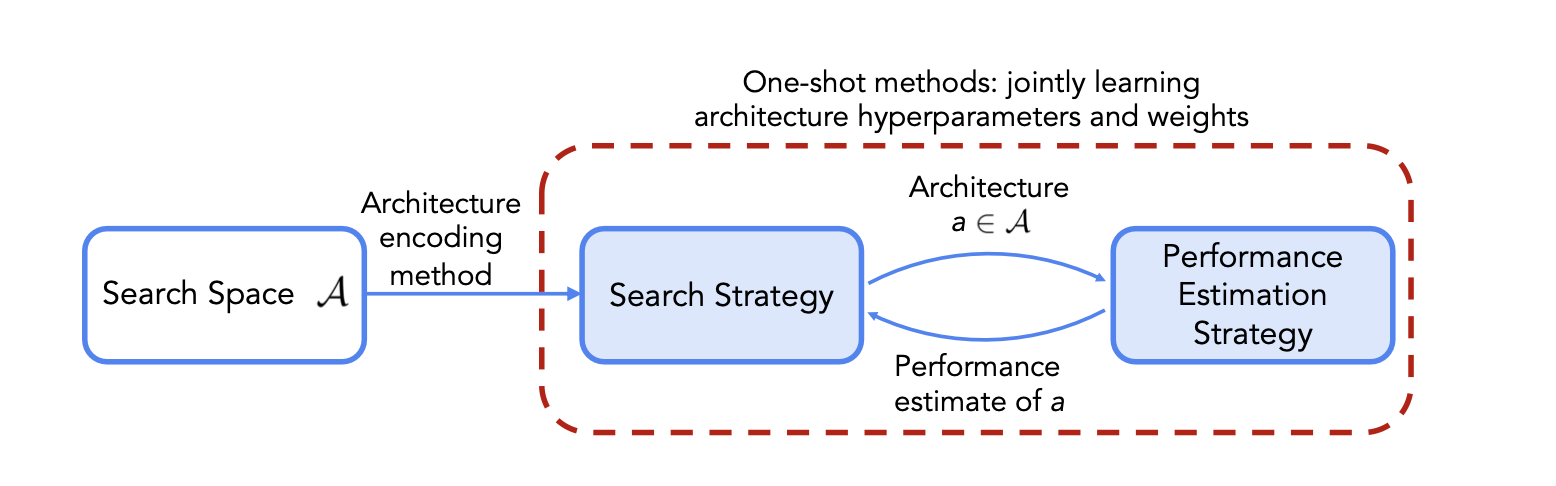
\includegraphics[scale=0.5]{figs/overview_nas.png}
	\refstepcounter{figure}
   	\addcontentsline{lof}{figure}{Figure~\thefigure: Overview of Neural Architecture Search}
	\label{fig: nas_overview}
	\parbox{\linewidth}{
	 \vspace{1em}
 	 {\small \textit{Figure \ref{fig: nas_overview}:} Overview of an architecture search process. The search strategy iteratively selects architectures from a predefined search space $\mathcal{A}$. The performance estimation strategy evaluates the model performance on the target dataset and then communicates back the performance to the search strategy.  \cite{white2023survey}.
	}
 	}
\end{figure}

\vspace{0.5em}
\noindent Next, we provide definitions of the terms and review the research progress of each domain.

\vspace{-1em}
\begin{description}[leftmargin=0cm, listparindent=\parindent]
	\item [Search Space] A search space defines a set of architectures that the search algorithm is allowed to select. The search space is often the first step when setting up \gls{nas} and perhaps is also the most essential step, because
		the design of the search space represents an important trade-off between human bias and efficiency of search: a
		smaller search space incorporating more prior human knowledge and involving more manual decisions will enable
		\gls{nas} algorithms to find high-performing architectures more easily, in contrast a larger space with more primitive
		building blocks provides higher odds of discovering truly novel architectures \cite{white2023survey}. Common  search
		spaces range in size from a few thousand to over $10^{20}$.	
	
		There are four major categories of search spaces in the \gls{nas} literature \cite{white2023survey}. We start with two types of search spaces that have relatively simple architecture topologies. The macro search spaces \cite{baker2017designing, kandasamy2018neural, zoph2017neural} encode the entire neural architecture at a high level. Typically, an entire architecture is often represented by a \gls{dag}, with nodes defining the operation types, like convolution or pooling,  and edges representing data flows. Each node is allowed to have distinct structures, such as convolution, pooling. As a result, macro search  spaces are highly flexible and possess high representation power. Another type is the chain-structured search spaces. As suggested by the name, chain-structured search spaces consist of neural networks that can be written as a sequence of operation layers. These search spaces often take state-of-the-art manual designs as the backbone. For example, there are several chain-structured search spaces based on the convolutional networks \cite{cai2018proxylessnas} or the transformer architectures \cite{xu2021nasbert}. 
		
		The third group is the cell-based search spaces, which perhaps are the most popular type of search spaces in \gls{nas} research. The cell-based search spaces are inspired by the fact that state-of-the-art human-designed architectures often consist of repeated blocks. For instance, the high-performing Transformer \cite{vaswani2017attention} contains 6 identical stacked encoder and decoder layers. Thus, instead of searching for the entire network architecture from scratch, \cite{zoph2018learning} propose to only search over relatively small cells  that comprises a set of operations, such as convolution. Then, the overall architecture can be formed by stacking the cells following a predefined skeleton. Building on this idea, \cite{zoph2018learning} proposes the first modern cell-based search space, NASNet, which comprises of two types of cells: the normal cell that preserves the dimensionality and the reduction cell that reduces the spatial dimension, as illustrated in Figure \ref{fig: cellss}. Since its emergence, many other cell-based search spaces have been developed. In general, these cell search spaces share a high-level similarity, but differ in the design of the fixed macro structure, the layout and constraints in the cells, and the choices of operations within the cells \cite{dong2020nasbench201, liu2018darts,  pmlr-v97-ying19a}. The cell-based approach significantly reduces the size and the complexity of the search space. However, it has been criticized for limiting the expressiveness of \gls{nas}, potentially hindering the discovery of highly novel architectures \cite{white2023survey}.	
		
		\begin{figure}[htbp]
			\centering
			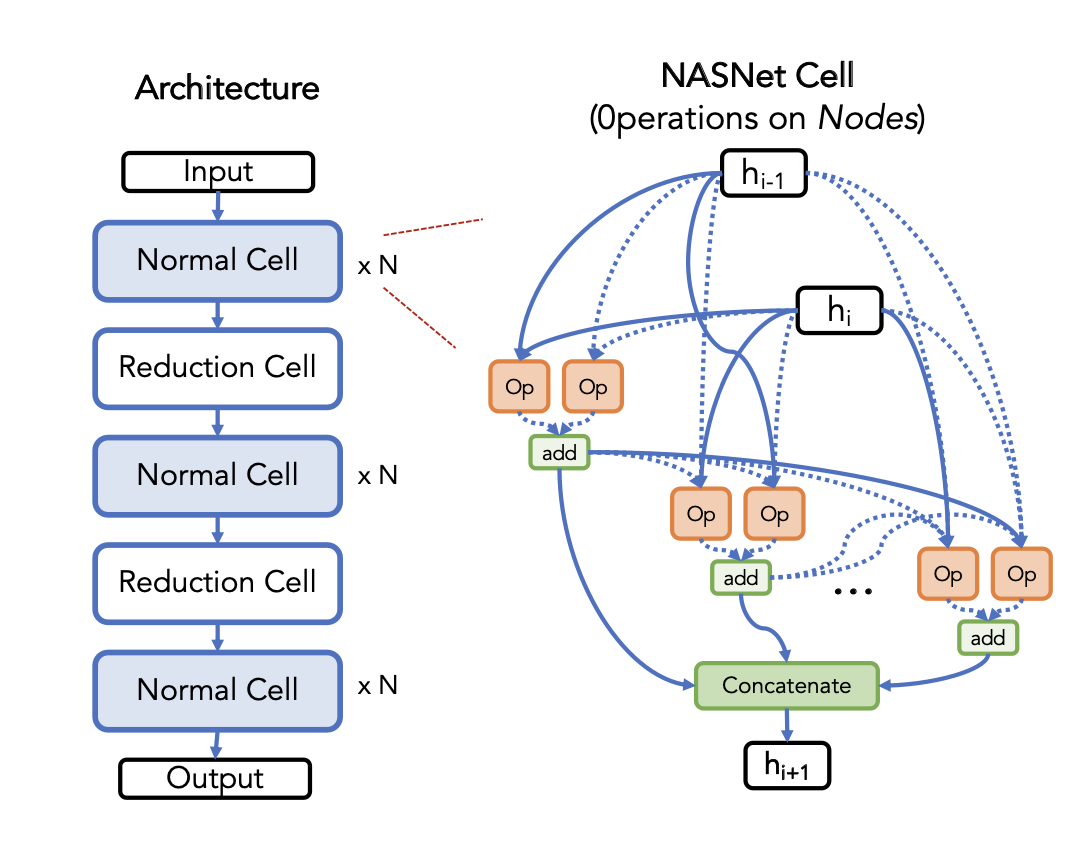
\includegraphics[scale=0.45]{figs/overview_cell_based_ss.png}
			\refstepcounter{figure}
   			\addcontentsline{lof}{figure}{Figure~\thefigure: Overview of Cell-based Search Space}
			\label{fig: cellss}
			\parbox{\linewidth}{
	 		\vspace{0.5em}
 	 		{\small \textit{Figure \ref{fig: cellss}:} Overview of a cell-based search space NasNet. The outer skeleton across cells (left) is fixed, and the operations, represented by nodes, within the cells are searchable (right) \cite{white2023survey}.
			}
 		}
		\end{figure}
		
		The last main category is the hierarchical search spaces. Different from the aforementioned types of search spaces that mostly have a flat representation, hierarchical search spaces involve designing patterns at different levels, where each higher-level pattern is often represented as a \gls{dag} of lower-level patterns \cite{christoforidis2021novel, liu2018hierarchical}.
		
	In addition to the architecture topology, another important design accompanying a search space is architecture encodings, because  many \gls{nas} algorithms require representations of the architectures to, for example, mutate an architecture or train a predictive model to extrapolate its performance. For search spaces that can be represented by a \gls{dag}, adjacency matrix is a commonly used encoding method. In addition, other encoding techniques, including graph-based encoding \cite{ning2020generic}, path-based encoding \cite{white2019bananas} and conditionally-structured encoding methods tailored for hierarchical search spaces have been proposed. \cite{white2020study} has shown that the effect of the encoding methods varies across different \gls{nas} subroutines.	
	  
	\item [Search Strategy] According to \cite{white2023survey}, there are generally two main categories of search strategies: black-box optimization based techniques and one-shot techniques. 
	 
		The black-box optimization based techniques largely overlap with another sub-area of AutoML: the hyperparameter tuning. Common techniques for hyperparameter tuning have been proven efficient for \gls{nas} as well, including reinforcement learning \cite{zoph2017neural, zoph2018learning}, evolutionary algorithms \cite{maziarz2018evo-nas,  real2019regularized}, gradient descent\cite{liu2018darts}, and etc. In particular, we take a close look at the search strategies based on Bayesian optimization, since they are closely related to the research question of this work. Initial Bayesian optimization based \gls{nas} approaches typically use the Gaussian Process (GP) as the surrogate model \cite{kandasamy2018neural}. However, these algorithms often demonstrate under-performance compared to their competitors due to several limitations: 1) search spaces are usually high-dimensional, non-continuous, and graph-like; 2) GPs requires custom distance metrics among architectures, which involves a time-consuming matrix inversion step. Besides, GPs are difficult to scale since the computation complexity grows cubically with the number of observations. To address these challenges, a new framework that using a neural predictor as the surrogate model for Bayesian optimization has been proposed and demonstrated strong performance \cite{ma2019deep, springenberg2016bayesian, white2019bananas}. We review this framework in details in Section \ref{sec:bananas}.
		
		The one-shot techniques are introduced to avoid training each architecture from scratch, The key idea is to train a \textit{supernetwork} that comprises all possible architectures in the search space as subnetworks. Once a supernet is trained, each architecture from the search space can be evaluated by inheriting the weights from the corresponding subnet within the supernet \cite{pmlr-v80-bender18a, liu2018darts}.
		
	\item [Performance Evaluation] The performance evaluation refers to the process of estimating the performance of architectures. In a NAS process, this estimated performance is communicated back to the search algorithm to guide the next search. The simplest performance estimation strategy is to fully train an architecture on the training data and then evaluate its performance on the validation data. However, training each architecture demands substantial computation resources and typically takes serval hours or days on a GPU. As a result, various approaches have been proposed to accelerate the evaluation of architecture performance. One popular line of work is to  predict the performance of neural networks before they are fully trained using zero-cost proxies \cite{pmlr-v139-mellor21a}.
	
	In this work, we primarily run experiments on the benchmark dataset NAS-Bench-201 \cite{dong2020nasbench201}, which offers queryable validation and test accuracies for all architectures in the search space and thereby eliminates the need to train neural networks when simulating \gls{nas} experiments. Hence, we provide only a brief overview of this aspect and refer the readers to \cite{white2023survey} for a comprehensive introduction to the performance evaluation techniques.	
	\end{description}}



\subsection{Bayesian Optimization and BANANAS}
\label{sec:bananas}
As briefly mentioned in Section \ref{sec: nas}, \gls{nas} search strategies based on Bayesian optimization with a neural network as the surrogate model have demonstrated strong performance. In particular, \cite{white2019bananas} identifies five critical components of this framework. After performing a thorough analysis on each component's effect towards the search performance, \cite{white2019bananas} develops the BANANAS algorithm based on both theoretical and empirical findings. This method is proven to be efficient and has achieved state-of-the-art performance on popular NAS benchmarks. 

This section offers a comprehensive review of the study. We start with the theoretical background and give an introduction into Bayesian optimization. Next, we walk through the five identified key components and provide a summary of the experimental findings.

Bayesian optimization \cite{Mockus1978} is a sequential decision-making process that seeks to find the global maximum (minimum can be seen as the negation of the maximum) of an unknown objective function $f : X \rightarrow R$ over an input space $X \subseteq R^d$. This objective function is often expensive to query. Therefore, a computationally efficient surrogate model is employed as a cheap approximation to the true objective. In a Bayesian optimization process, the surrogate, usually a Gaussian Process or a Parzen-Tree Estimator \cite{bergstra2011algorithms}, also encodes the prior belief over the objective function. At each iteration, the surrogate model updates the prior with the observations and forms a posterior probabilistic distribution of $f$. Then, the acquisition function, another key component that trades off exploration and exploitation in the process, evaluates a set of candidates based on the posterior distribution and picks the data point that gives the largest acquisition score for next query. Algorithm \ref{alg:BO} outlines this procedure.

\begin{algorithm}[t]
  \caption{Bayesian Optimization}
  \label{alg:BO}
  \begin{algorithmic}[1]
  \textbf{Input:} surrogate model $\mathcal{M}$, acquisition function $\phi$, objective function $\myfunc{f(\cdot)}$, number of iterations $T$. \vskip
  
  \STATE Initialize the set of observations: $D \leftarrow \emptyset$
  \FOR {$t$ in $1,...,T$}
  		\begin{enumerate}
    	    \itemsep0em 
			\item Fit surrogate model $\mathcal{M}$ to current observations set $\mathcal{D}_{t-1}$.
			\item Evaluate acquisition function and select the next point for query: \newline
				  $x_t = \operatorname*{argmax}_{x \in X} \; \phi(x, \; \mathcal{M})$	
			\item Query the objective function: $y_t = f(x_t)$
			\item Update the observations set: \mathcal{D}_t \leftarrow \mathcal{D}_{t-1} \cup \{(x_t, y_t)\}
		\end{enumerate}
  \ENDFOR
  \STATE \textbf{Output:} $x^*=\operatorname*{argmax}_{t=1,...,T} f(x_{t})$    
 \end{algorithmic}
 \end{algorithm}

\vspace{0.5em}
The acquisition function adopted in the original paper \cite{Mockus1978} is the \gls{ei}. Other popular alternatives include: \gls{ts}, \gls{its}, \gls{ucb}, and \gls{pi}. Different acquisition functions typically favor exploration and exploitation differently. Nevertheless, \cite{agnihotri2020exploring} shows that \gls{ei} is competitive in reaching the optimum value with comparably few iterations. 

\begin{figure}[htbp]
	\centering
	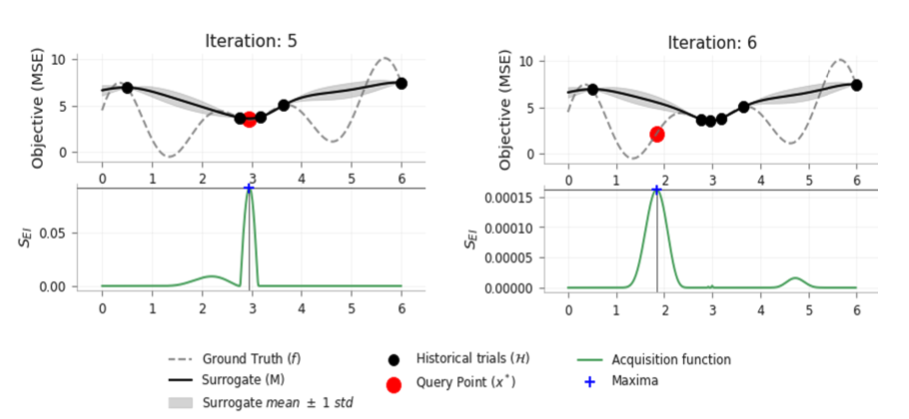
\includegraphics[scale=0.4]{figs/overview_bo.png}
	\refstepcounter{figure}
   	\addcontentsline{lof}{figure}{Figure~\thefigure: Illustration of Bayesian Optimization}
	\label{fig: bo}
	\parbox{\linewidth}{
	\vspace{0.5em}
 	{\small \textit{Figure \ref{fig: bo}:} Example of Bayesian optimization with Gaussian Process as the surrogate and \gls{ei} as the acquisition function to explore the minimum of the objective function \cite{agnihotri2020exploring}.
 	}
 	}
\end{figure}

Next, we return to the NAS framework "Bayesian optimization + neural predictor". Now it becomes obvious that this framework is essentially an optimization task that searches the maximum value. The objective function in this context maps each architecture in the search space to its corresponding validation accuracy. The surrogate model is a neural network and takes architectures or their encodings as the inputs. \cite{white2019bananas} identifies five critical components within the framework, listed as follows:

\begin{description}[leftmargin=0cm, listparindent=\parindent]
	\item [Architecture Encoding] This item refers to obtaining a vector representation of the architectures. Previous work often encode architectures using an adjacency matrix based approach, where nodes are assigned with an arbitrary ordering  and then binary features for all edges in the \gls{dag} are set to form the final representation.	Notably, the resulting representation of a specific architecture is not deterministic since the encoding  relies on an arbitrary indexing of the nodes. 
 
	In contrast, \cite{white2019bananas} proposes a novel path-based encoding mechanism with optional path truncation. This method simply checks if a path from the input node to the output node, expressed in terms of operations (e.g., input $\rightarrow$ 1$\times$1 conv $\rightarrow$ 3$\times$3 pool$\rightarrow$ output), is present in an architecture. The final encoding is a binary vector indicating which of the possible paths within a cell are present in the architecture. In this way, an architecture is always mapped to the same (though not necessarily unique) path encoding. Experiments show that the path-based encoding substantially increases the performance of neural predictors.
	
	\item [Neural Predictor] This item is about choosing an appropriate neural network for surrogate, which maps architecture encodings to the corresponding performances. To select the optimal neural predictor, several candidates are examined, include VAEs, GCNs, and FNNs with either adjacency matrix or path-based encoding. These predictors are first trained on a dataset, which is formed by randomly sampling a set of architectures and their corresponding validation accuracies from the search space, and then compared on a holdout set. Among all tested neural predictors, FNNs with path encoding demonstrates the strongest performance.
	 
	\item [Uncertainty Estimation] Uncertainty estimates are required to form the probabilistic distribution. In particular, Bayesian neural networks (BNNs) and an ensemble of \gls{fnns} are investigated. For BNNs, the posterior distribution is inferred over the network weights. For \gls{fnns}, the predictive distribution is simply modeled as a Gaussian, parameterized by the mean and standard deviation of the ensemble base learners' predictions. The results show that an ensemble of even only 3 to 5 neural networks in general yields more reliable uncertainty estimates than BNNs.
	
	\item [Acquisition Function] In the experiments, five commonly used acquisition functions are examined: \gls{ts}, \gls{its}, \gls{ucb}, \gls{pi}, and \gls{ei}. Each function is adapted to the Gaussian assumption, thereby requiring only the mean and standard deviation estimates to compute the acquisition scores. The experiments show that overall \gls{its} yields the best performance among all the options, although the marginal outperformance is subtle. The results indicate that the acquisition function does not have as significant impact on the search performance as the other examined components in the framework.
		
	\item [Acquisition Optimization] In each iteration of the Bayesian optimization, the goal is to select a candidate from the search space that maximizes the acquisition score. Evaluating the acquisition function for every architecture available in the search space is computationally infeasible, therefore \cite{white2019bananas} proposes to create a set of 100 to 1000 candidates and then choose the architecture with the maximal acquisition score in this set. Specifically, \cite{white2019bananas} explores various approaches for creating this candidate set. The simplest and most natural way is to draw architectures at random. Consider that architectures close in edit distance to those used for training the surrogate model are likely to have more accurate estimates, an alternative is a mutation-based sampling approach, where the candidate set is created via local search by randomly modifying an operation or an edge of the best-performing architectures that have been evaluated so far. In additional, \cite{white2019bananas} also examines a hybrid approach that combines random search with mutation-based search. Their experiments show that the mutation-based approach outperforms its competitors and suggest it is better to search locally rather than globally.
\end{description}}

Finally, the best components found in the aforementioned analyses are transformed into the BANANAS algorithm. Considering its strength in both prediction and uncertainty quantification, an ensemble of \gls{fnns} using the path encoding is employed as the surrogate model and typically uncertainty is modeled as a Gaussian distribution. In addition, \gls{its} with a mutation strategy for acquisition (Figure \ref{fig: bananas}). 

\begin{figure}[t]
	\centering
	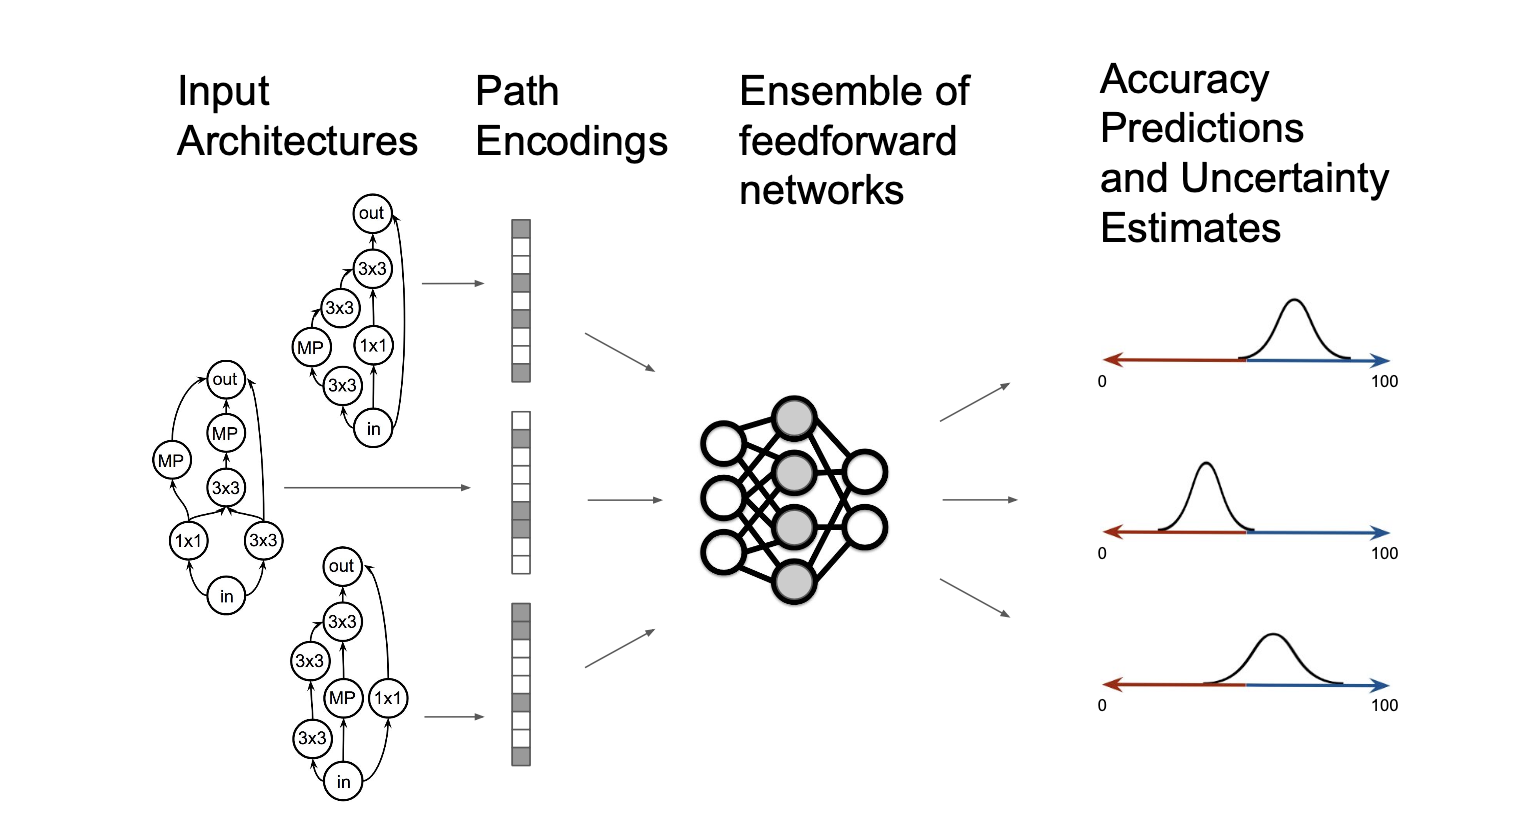
\includegraphics[scale=0.48]{figs/overview_bananas.png}
	\refstepcounter{figure}
   	\addcontentsline{lof}{figure}{Figure~\thefigure: Diagram of the BANANAS framework}
	\label{fig: bananas}
	\vspace{0.5em} 
	\\
 	{\small \textit{Figure \ref{fig: bananas}:} Diagram of the BANANAS framework \cite{white2019bananas}.}}
\end{figure}

\section{Uncertainty Quantification Methods}
While BANANAS employs a relatively simple method for uncertainty estimation, there are many commonly used \gls{uq} techniques that are generally more theoretically grounded and sophisticated. In this section, we review some of these \gls{uq} methods and explain the rationale for choosing \gls{cp} for the development of our approach. Despite not directly tied to this work, this thesis aspires to offer a comprehensive overview of common \gls{uq} techniques applied in deep learning.

Formally, \gls{uq} is the science of quantitative characterization and estimation of uncertainties in both computational and real world applications. The source of uncertainty can be categorized into two types:

\begin{description}[leftmargin=0cm]
\item[Aleatory Uncertainty:] also known as data uncertainty, refers to uncertainty that arises due to inherent noices or randomness in a system and can not be reduced. \item[Epistemic Uncertainty:] also known as model uncertainty, refers to uncertainty that arises due to lack of knowledge, and can be reduced by better modeling or collecting more data.
\end{description}

A family of methods for quantifying uncertainty directly model the full predictive distribution of the output, i.e., $p(y \mid x)$. One example is the Gaussian Process, which is typically parameterized by a kernel function and the predictive inference can be obtained in an analytical manner based on the observations. Another important example is the Bayesian Neural Network \cite{kendall2017uncertainties, neal1996bayesian}, in which each weight in the network is seen as a random variable rather than a single number. In practice, however, the posterior distributions over weights are intractable due to the integral operation and the high dimensionality. Therefore, the posterior can only be approximated using e.g.,  variational inference or Monte-Carlo sampling methods \cite{neal1996bayesian, springenberg2016bayesian}, both requiring multiple forward passes through the network. 

Like the inference stage in BNNs, some methods also rely on aggregating statistics from sub-networks, such as Monte-Carlo Dropout \cite{gal2016dropout} and Deep Ensemble \cite{lakshminarayanan2017simple}. The idea of Monte-Carlo Dropout is to apply \textit{dropout}, a regularization technique often used for preventing overfitting during the training time by randomly deactivating neurons, also at the inference time. Specifically, the model run multiple times on the same input with stochastically deactivated neurons and thereby get  different predictions, which are seen as the approximation to the distribution of the output. Deep Ensemble involves using a network that outputs two values in the final layer, corresponding to the predicted mean $\mu(x)$ and the variance $\sigma^2(x)$, respectively. This neural network is typically trained by minimizing a custom loss function in which $\mu(x)$ and $\sigma^2(x)$ have opposing effects. To avoid overfitting and lower estimation variance, multiple instances of the neural network are initialized with different weights and trained independently. Then, the final estimates of $\mu(x)$ and $\sigma^2(x)$ are obtained by aggregating the predictions from all these sub-networks. 

Another popular approach is Quantile Regression (QR) \cite{koenker1978regression}. Instead of modeling the full distribution, QR only models a sequence of discrete quantiles of the output. We present QR with more details in Section \ref{sec:cp}. 

However, these \gls{uq} techniques face several challenges in practice. Some methods require multiple forward propagations either during the training or inference time, such as BNNs, Deep Ensemble. This is in general computationally intensive and may cause the models difficult to scale and consequently limit their applications for real-time prediction or in an online setting. In addition, the inference quality of BNNs depends on if the prior of weights is correctly specified, which demands expertise and can potentially introduce human bias. On the other hand, some models are pre-trained and are only accessible via API, making intervening the training process practically infeasible \cite{mossina2024CVPR}. Moreover, pre-trained models developed using certain datasets may struggle to generalize across different domains or contexts. 

\vspace{0.3cm}
Post-hoc uncertainty calibration techniques can serve as an effective approach in the restricted scenarios described above. Instead of assessing and measuring uncertainties on the model level, calibration targets on adjusting a model's predicted probabilities to make the reported uncertainties better aligned with the actual likelihoods.

Platt Scaling \cite{platt1999probabilistic} probably is the first calibration technique applied in modern machine learning. This method is introduced in the context of Support Vector Machines and is intended for classification problems. For regression problems, one widely used calibration technique is Isotonic Regression \cite{niculescumizil2005predicting}, a technique of fitting a step-wise line to a sequence of observations such that the fitted line is non-decreasing (or non-increasing) everywhere. The monotonicity of the resulting line allows to preserve the order of predicted quantiles, making this method appealing for uncertainty calibration. For example, \cite{pmlr-v80-kuleshov18a} show that accurate uncertainty estimates can be obtained by training a recalibrator on a holdout dataset using isotonic regression.

Recently, Conformal Prediction (CP) \cite{shafer2008tutorial, vovk2005algorithmic} is emerged as a new, distribution-free framework for uncertainty quantification. This technique has been widely adopted for both classification and regression problems despite of its relatively short history. Fundamentally, CP serves as a model-agnostic wrapper and can be applied with any arbitrary prediction algorithms. It works by constructing a prediction interval (for regression) or a set of possible values (for classification) that will cover the true value with a predefined probability. The fact that \gls{cp} is applied in a post-hoc fashion with minimal assumptions enables it to capture both aleatoric and epistemic uncertainties \cite{mossina2024CVPR}. Moreover, like most other post-hoc calibration methods, \gls{cp} offers the advantage of being light-weighted with little overhead to implement. We present a thorough introduction into the \gls{cp} framework in the following section.

\section{Conformal Prediction}
\label{sec: reviewCP}
\subsection{Theoretical Background}
We start by introducing the concept of \textit{exchangeable data}, which is an key prerequisite for understanding \gls{cp}.
\newline

\noindent
\textbf{Definition (Exchangeability):}  
A sequence of random variables \( (Z_1, Z_2, \dots, Z_n) \) is said to be \textit{exchangeable} if its joint probability distribution is invariant under any permutation of the indices. That is, for every permutation \( \pi \) of the set \( \{1, 2, \dots, n\} \),
\[
P(Z_1, \dots, Z_n) = P(Z_{\pi(1)}, \dots, Z_{\pi(n)})
\]

\noindent Note that exchangeability allows for dependencies among data points, as long as the joint distribution is invariant under any permutation. Accordingly, it is weaker than the i.i.d. assumption. Then, the goal of \gls{cp} can be formally defined as: 
\newline

\noindent
\textbf{Definition (Conformal Prediction):}  Let \(B = \{(x_1, y_1), \dots, (x_n, y_n)\}\) be a bag of observed examples from an exchangeable joint distribution $\mathbb{P}_{X,Y}$, with $X \subset R^d$ representing some features and  $Y$ the target variable. Given a new unseen input \(x_{n+1}\), conformal prediction constructs a prediction region \( \mathcal{C}_n^\tau(x_{n+1}) \) using a \textit{conformity score function} such that
\vspace{0.7em}

\begin{equation}
\mathbb{P}\left( y_{n+1} \in \mathcal{C}_n^\tau(x_{n+1}) \right) \geq 1 - \tau
\vspace{1em}
\label{eq: finitecp}
\end{equation}

\noindent
where \( \tau \in (0, 1) \) is the predefined nominal mis-coverage rate. This probability is also known as the \textbf{finite-sample validity} property of \gls{cp} and is taken over the joint distribution of all \(n + 1\) samples. Moreover, the prediction regions for different $\tau$ should be nested. That means, if  $\tau_1 \ge \tau_2$, then $1 - \tau_1$ is a lower confidence level than $1 - \tau_2$ and we have $ \; \mathcal{C}_n^{\tau_1}(x_{n+1}) \subseteq \mathcal{C}_n^{\tau_2}(x_{n+1})$ \cite{shafer2008tutorial}.  

\vspace{0.7em}
\textbf{Conformity score function} is a real-valued function  measures how dissimilar an example is compared to the examples in the bag $B$. Now generalizing this setting to a supervised learning framework, a predictive algorithm $f$ that maps features to the target variable naturally induces a conformity measure. Specifically, we denote $d(z_{n}, B), \; z_{n} = (x_{n}, y_{n})$ a conformity function, such that a higher value indicates the greater a point deviates from the samples in $B$. Denote $\hat{f}_n$ the predictor trained on the $n$ existing observations in the bag. Since the prediction rule is learnt from examples in the bag, $\hat{f}_n$ is then encoded in $B$ in this distance expression. When using $\hat{f}_n$ to generate a point prediction for $x_{n+1}$, intuitively, the distance between the predicted value $\hat{f}_n(x_{n+1})$ and the true value $y_{n+1}$ (after the value is revealed), should inform how different $z_{n+1}$ is compared to the existing examples in the bag. Consequently, with a distance-like conformity score function, the prediction set for an unseen data point $x_{n+1}$ sampled from the same distribution should be constructed by collecting all values such that $d(\cdot, B)$ smaller than a threshold, i.e., points that are expected to lie within a certain distance from the true value.

\begin{figure}[H]
	\centering
	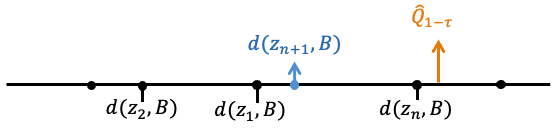
\includegraphics[scale=0.4]{figs/cp_symmetry.png}
	\refstepcounter{figure}
   	\addcontentsline{lof}{figure}{Figure~\thefigure: Illustration of Symmetrical Data}
	\label{fig: cpsymmetry}
	\vspace{0.5em} 
	\\
 	{\small \textit{Figure \ref{fig: cpsymmetry}:} Illustration of Symmetrical Data in Conformal Prediction}}
\end{figure}

\vspace{0.5em} 
An important intuition behind selecting the threshold that eventually defines the prediction region is \textit{symmetry}, that is, all data points are treated symmetrically within the \gls{cp} framework \cite{angelopoulos2021gentle}. Suppose $d(z_1, B), \, d(z_2, B), \; ... \; ,d(z_n, B)$ is a sequence of observations in the form of conformity scores, the exchangeability assumption implies that the rank of a new data point $d(z_{n+1}, B)$ is uniformly distributed over the observed values. Figure \ref{fig: cpsymmetry} illustrates the concept of symmetry. As a result, the $(1 - \tau)$-th quantile of all the conformity scores is a natural answer to achieve the coverage probability stated in Formula \ref{eq: finitecp}. Recall that the coverage probability is achieved on the $n+1$ samples, the quantile value should be adjusted with a finite-sample correction, resulting in a threshold that is exactly equal to 

\begin{equation}
\vspace{0.7em}
\frac{\lceil(1 - \tau)(n + 1)\rceil}{n}\text{-th quantile of conformity scores}
\label{eq:cpquantile}
\vspace{0.7em}
\end{equation}

\noindent
\textbf{Finite-sample Validity} Note that the coverage guarantee provided by the \gls{cp} framework is marginal, meaning it holds on average over all data points. This is a significantly weaker requirement than the conditional coverage, which requires the guarantee to hold for each individual input (Figure \ref{fig: coverage}). Nevertheless, \gls{cp} remains a powerful tool for uncertainty quantification, because the finite-sample coverage is valid regardless of the size of the observations bag or the choice made for the underlying prediction algorithm or the conformity score function. Under the distance interpretation presented earlier, a smaller score indicates that the new sample conforms more closely with the existing observations. In such case, the function is also referred as a negatively-oriented score and, to be precise, it is actually a non-conformity measure. A positively-oriented one also works in practice, provided with correct modifications. In the context of this work, for simplicity, we always refer to a negatively-oriented score with distance-like interpretations, unless otherwise specified.

\begin{figure}[htbp]
	\centering
	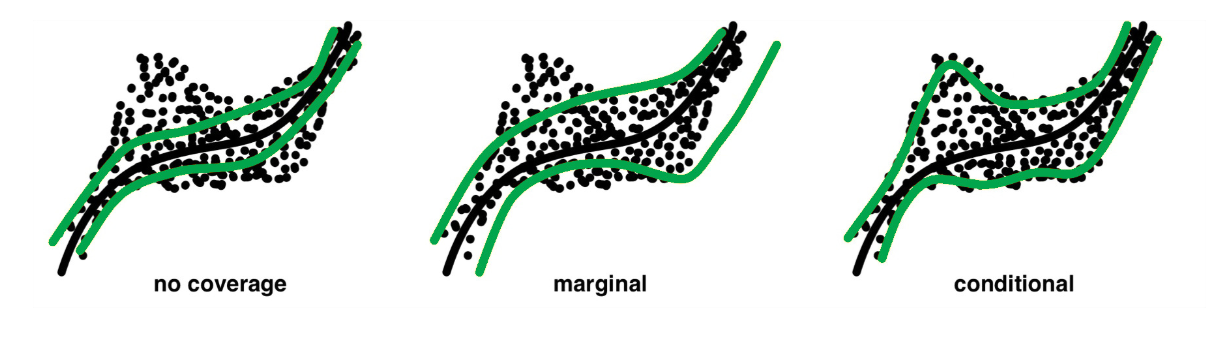
\includegraphics[scale=0.28]{figs/overview_coverage.png}
	\refstepcounter{figure}
   	\addcontentsline{lof}{figure}{Figure~\thefigure: Example of Different Coverage Types}
	\label{fig: coverage}
	\vspace{0.5em} 
	\\
 	{\small \textit{Figure \ref{fig: coverage}:} Example of Different Coverage Types}}
\end{figure}

Although coverage is guaranteed for any conformity scoring function, this scoring method is actually an important engineering decision and has significant impact on the effectiveness of the constructed prediction set. Imagine a classification problem, if we produce a set that contains all possible classes, then surely the true label is covered by the set. However, such prediction set is neither informational nor actionable, offering little value in application. This concern naturally introduces a second evaluation criterion for \gls{cp}: while ensuring coverage guarantees, ideally the yielded prediction set should be as compact as possible.

\vspace{1.5em}
\noindent \textbf{A Link to Hypothesis Testing} It is noticeable that \gls{cp} exhibits a couple of structural similarities to hypothesis testing, which is a fundamental tool in statistical inference and perhaps sounds more familiar to most ears. For example, both methods involves producing an interval and relying on a certain threshold to make decisions. In fact, these terms are often used interchangeably in many research work. This motivates us to seek an interpretation of the \gls{cp} framework through the hypothesis testing perspective, such that we gain a deeper and clearer understanding of \gls{cp}.

\begin{table}[t]
    \centering
    \refstepcounter{table}
   	\addcontentsline{lot}{table}{Table~\thetable: Comparison between Conformal Prediction and Hypothesis Testing}
   	
 	{\small \textit{Table \ref{tab:cpht_comparison}:} Comparisons between conformal prediction and hypothesis testing}
	\vspace{0.7em}

    \renewcommand{\arraystretch}{1.2}
   	\begin{tabular}{| m{1.5cm} | m{6cm} | m{5.8cm} |}
    \hline
    &\textbf{Conformal Prediction} & \textbf{Hypothesis Testing} \\
    \hline
    \textbf{Input} & nominal mis-coverage level $\tau$ & significance level $\alpha$ \\
    \hline
    \textbf{Decision rule} & compare the conformity score of a data point against the quantile value & compare $p$-value, which is an empirical measure, to the significance level \\ 
    \hline
	\textbf{Output} & prediction interval offering marginal coverage with probability $1 - \tau$ & confidence interval that contains the true parameter value with probability $1 - \alpha$  \\
	\hline        		
    \end{tabular}
    \label{tab:cpht_comparison}
\end{table}
	  	
Both methods take a predefined value ranging from 0 to 1 as input. In the context of \gls{cp}, this value is often interpreted as mis-coverage rate or error rate, referring to the probability that the prediction region fails to cover the true value. The corresponding concept in hypothesis testing is the significance level, referring to the probability of rejecting the null hypothesis when it is actually true. Table \ref{tab:cpht_comparison} offers a summary of the terms used in \gls{cp} alongside with their parallel in hypothesis testing.

Intuitively, we can think \gls{cp} as running a sequence of hypothesis tests for a given new point $x_{n+1}$, with each testing a candidate value for $y_{n+1}$, denoted as $\tilde{y}$. Hypotheses are defined as: \\

\vspace{-0.3em}
\indent $H_0$: The new example $(x_{n+1}, \; \tilde{y})$ conforms to the existing observations. \\
\indent	$H_1$: The new example $(x_{n+1}, \; \tilde{y})$ does not conform to the existing observations. \\
\vspace{-0.3em}

\noindent After obtaining conformity scores for all $n+1$ data points, in this context, the fraction of conformity scores that is larger than that for $(x_{n+1}, \tilde{y})$, or equivalently, the complement of the quantile of the conformity score for $(x_{n+1}, \tilde{y})$, can be seen as a $p$-value. If the $p$-value exceeds the predefined significance level, we fail to reject the null hypothesis, and consequently, this candidate $\tilde{y}$ should be included in the prediction set \( \mathcal{C}_n^\tau(x_{n+1}) \). In fact, this interpretation from the hypothesis testing perspective reflects the core idea of the approach known as full conformal prediction, which we formally introduce in the following section.

\subsection{Full Conformal Prediction}
In fact, conformal prediction is originally designed for a transductive setting, in which the prediction for a test point is generated using the full dataset available at the inference time \cite{gammerman1998learning}. Hence, this transductive \gls{cp} framework is also known as \gls{fcp}. Typically, new observations are revealed sequentially, which means, after the prediction is generated for a test point, its true value is observed before the next prediction is made. 

The core idea for constructing a prediction set for a given test point $x_{n+1}$ is to iterate over all possible values in the target variable space. As performed in hypothesis testing, for each candidate $\tilde{y}$, a conformity score and its corresponding $p$-value will be calculated. Specifically, the conformity score for candidate $\tilde{y}$ is computed in a way where a prediction rule $\hat{f}_{\tilde{y}}$ is learnt using all pairs in the bag \(B = \{(x_1, y_1), \dots, (x_n, y_n), (x_{n+1}, \tilde{y})\}\), then the conformity score is computed as a distance measure between $\hat{f}_{\tilde{y}}(x_{n+1})$ and $\tilde{y}$. This process is repeated for all available candidates and the prediction set is constructed by collecting every $\tilde{y}$ with which the null hypothesis in the previous sub-section can not be rejected. Typically, if the target variable space is continuous, the space is first discretized to form a finite grid, then each element in the set can be checked, e.g., using grid search \cite{angelopoulos2021gentle}.

Moreover, after the true value $y_{n+1}$ is revealed, the underlying bag of observations gets updated by including this data point, and the above procedure needs to start from scratch when generating prediction for each new test point. Suppose the target variable space has a size of $K$, to generate prediction regions for $m$ unseen instances, the underlying prediction algorithm should fit for $K \cdot m$ times. Clearly, \gls{fcp} in general is extremely computationally expensive, which renders the application of \gls{fcp} highly unsuitable for training-intensive works, such as with neural networks.

\subsection{Extensions of Conformal Prediction}
Since the transductive version of \gls{cp} that was first proposed in \cite{gammerman1998learning}, several variants of \gls{cp} have been developed with different computational complexities, formal guarantees, and practical applications.

To address the aforementioned inefficient computation problem of \gls{fcp}, Split Conformal Prediction (\gls{scp}), also known as Inductive Conformal Prediction (ICP), was first introduced in \cite{papadopoulos2002inductive} by replacing the transductive inference with inductive inference, aiming to learn a general prediction rule about the data using the observed records. Then, this rule can be applied directly to obtain predictions when new data arrives in sequence, without re-using the training data and retraining the model repeatedly. The main concept involves splitting the data into two non-overlapping subsets, designated for training and calibration, respectively. A predictive model is fit exclusively on the training set, then (non-)conformity scores are computed using the calibration set to obtain the quantile value that determines the width of the prediction interval. Due to its simplicity and computational efficiency, \gls{scp} is one of the most commonly used techniques in the \gls{cp} family. Since  \gls{scp} is an important component in the methodological framework proposed in this work, we introduce \gls{scp} in details with pseudo-code in Section \ref{sec:scp}.

\vspace{0.5em} 	
Apart from hight computational cost, \gls{cp} still faces several challenges in practice: 
\vspace{0.2em} 

\noindent \textbf{Distribution/Covariate Shift:} The finite-sample validity offered by \gls{cp} depends on exchangeable data. However, the key assumption of exchangeability is often violated in real-world applications, in which the underlying data generation process might vary over time. For example, in finance market behavior can shift drastically in response to major world events. \\
 \noindent \textbf{Adaptivity:} The conformity score adopted in the original \gls{scp} work is based on the  absolute residual $|y - \hat{y}|$, which leads to a prediction interval with fixed width and does not adapt to the intrinsic complexity of the specific test example.
\vspace{0.5em} 

Various \gls{cp} algorithms have been developed to address limitations and broaden application domains. These extended algorithms can be mainly categorized into three types in accordance with the structural components in a \gls{cp} framework. 
\vspace{0.5em} 

One line of work focus on the coverage rate. Instead of using a static predefined mis-coverage rate $\tau$ for computing the quantile of conformity scores, \cite{gibbs2021adaptive} develops a method called \textit{ACI} where the applied mis-coverage level is dynamically adapted based on empirical mis-coverage frequency of previous prediction sets. This approach is applied in an online setting. At each time $t$, the applied mis-coverage rate $\tau_t$ is derived by decreasing (resp. increasing) the current value if the prediction sets were historically under-covering (resp. over-covering). The amplitude of rate adjustment is jointly controlled by the pre-specified learning rate and the empirical mis-coverage level. In this setting, the empirical mis-coverage frequency of previous examples serves as a signal of distribution shift or violation of exchangeability. \cite{gibbs2021adaptive} show that \textit{ACI} is capable of forming prediction sets that are robust to changes in the underlying data distribution. \cite{zaffran2022adaptive} extends \textit{ACI} to time-series data and introduce \textit{AgACI}, which is a parameter-free variant of \textit{ACI} that uses online expert aggregation to adaptively combine multiple ACI experts. In contrast to \textit{ACI}, where the learning rate should be carefully chosen in advance, \textit{AgACI} leverages a number of $k$ experts working with different learning rates, and automatically learns the optimal learning rate by aggregating across experts such that each expert's contribution is proportional to their corresponding performances over previous iterations. \cite{zaffran2022adaptive} show \textit{AgACI} demonstrates strong performance and produces tighter, well-calibrated prediction intervals consistently.  

\vspace{0.3em} 
Another line of work strives to find suitable and efficient conformity score functions tailored for specific tasks. For example, \cite{lei2018distribution} introduces a simple score for regression that accounts for heteroskedasticity, thus offering local adaptivity. \cite{romano2020classification} proposes a novel conformity score crafted for multi-label classification tasks. While providing marginal coverage, this score also demonstrates full adaptiveness to data complexities and enhances the approximated conditional coverage. In parallel, \cite{romano2019conformalized} develops a conformity score that involves both upper and lower bounds corresponding to a given coverage rate, enabling to combine the strengths of quantile regression and conformal prediction. Furthermore, \cite{xie2024boosted incorporates a boosting procedure between the training and calibration steps in order to enhance an arbitrary score function.

\vspace{0.3em} 
The underlying prediction algorithm also plays an important role in \gls{cp}, since the trained predictor serves as an approximation of the real data generation process and determines the base from which intervals are constructed. \gls{scp} fits the predictor only once, however potentially at a cost of training accuracy and statistical efficiency, since both training set and calibration set only see a subset of samples. One way to address this challenge is combining conformal prediction with techniques like cross-validation\cite{vovk2015cross}, Jackknife+ \cite{barber2020jackknife} and bootstrapping \cite{kim2020predictive}, such that all data points are used for both training and calibration, with only a limited number of model fits. 

\vspace{0.3em} 
In addition, there are works beyond the above three categories. Some works boost prediction reliability through enhancing the datasets. \cite{StutzTMLR2023} proposes a CP algorithm targeted on a special classification case where the ground-truth is ambiguous and consequently cause a biased distribution in manually-annotated labels. This method approximates the true distribution of labels by resampling data points using Monte-Carlo sampling method. \cite{Shanmugam2025TTA} proposes to integrate a test-time data augmentation into \gls{cp} to reduce prediction set size and improve stability. Moreover, Conformal Risk Control \cite{angelopoulos2022conformal} also emerges as an important extension of \gls{cp} that not only provides distribution-free coverage guarantees but also explicitly controls risk. It is achieved by replacing the mis-coverage probability in normal \gls{cp} with the expected value of a custom loss function. The prediction set is then bounding to a predefined loss tolerance instead of a mis-coverage rate. Several works have adopted this risk-control approach such as \cite{mossina2024CVPR}.


% chapter 3
\chapter{Methodology}
\label{ch3}
Despite of its provable strength, \gls{bananas} assumes a Gaussian distribution for measuring uncertainty. However, this assumption does not necessarily hold in real world. To mitigate the potential limitations caused by inaccurate uncertainty estimates, this work proposes a new framework, \gls{bananascp}, that integrates a conformal prediction-based uncertainty calibration process into \gls{bananas} in an online setting. To begin, we present an algorithm outlining the overall procedure of \gls{bananascp} in Section \ref{sec:overview}, and give detailed descriptions of each methodological step in the following sections. 

\section{The BANANAS--CP Framework}
\label{sec:overview}

Refer to Section {\ref{sec:bananas} for a detailed introduction of the original \gls{bananas} algorithm. In this section, we emphasis the key ideas of the uncertainty calibration mechanism, which corresponds to Step 1 to 6 of the inner iteration in Algorithm {\ref{alg:OCP}.

\begin{algorithm}[htbp]
  \caption{The BANANAS--CP Framework}
  \label{alg:OCP}
  \begin{algorithmic}[1]
    \textbf{Input - NAS parameters:}
    search space $\mathcal{A}$, evaluation dataset $\mathcal{D}$, exploration budget $T$, 
    the number of initially sampled architectures $t_{0}$, acquisition function $\phi$, surrogate model $\mathcal{M}$ that approximates the true objective function, function $\myfunc{f(\cdot)}$ returning validation error of an architecture after training. \newline
    \textbf{Input - Calibration parameters:} a function $\myfunc{C(\cdot)$ to create calibration set, a non-conformity score function $\myfunc{s(\cdot)}$, and an array of desired quantile levels $q$. \vskip
    \vspace{0.7em}
    \STATE Draw $t_{0}$ architectures {$\{a_{1}, a_{2},..., a_{t_{0}}\}$} uniformly at random from $\mathcal{A}$ and train each individual architecture on $\mathcal{D}$.
    \vspace{0.3em}
   	\STATE $\mathcal{A}_{t_{0}} \leftarrow{\{a_{1}, a_{2},..., a_{t_{0}}\}$},
   	\vspace{0.3em}	
    \FOR {$t$ in $t_{0}+1,...,T$}
    	\begin{enumerate}
    	    \itemsep0em 
			\item Apply $\myfunc{C(\cdot)$ and split all evaluated architectures into two disjoint datasets; use them as a training set $\mathcal{A}_{t, train}$, and a calibration set $\mathcal{A}_{t, cal}$.
			\item Train the surrogate model $\mathcal{M}_{t}$ on $\{a, \myfunc{f(a)}\}, a \in \mathcal{A}_{t, train}$ using the path encoding to represent each architecture. 
			\item Compute the conformity scores $\myfunc{s}$ on $\mathcal{A}_{t, cal}$.
			\item Generate a set of candidate architectures from $\mathcal{A}$. 
			\FOR {each $a_{i}$ in candidates}
				\begin{enumerate}
				\itemsep0em 
				\item Estimate the value for each quantile level $q_i$ in $q$ and calibrate using conformity scores computed in the previous step, with $q_i$ implying a mis-coverage rate $2q_i$ or $2(1-q_i)$ for conformal prediction.
				\item Fit a distribution $F_{i}$ based on the estimated quantile values.
				\item Compute the acquisition score $\myfunc{\phi(a_{i})}$.
				\end{enumerate}
			\ENDFOR
			
			\item Denote $a_{t}$ as the candidate architecture with maximum $\myfunc{\phi(a)}$; evaluate $\myfunc{f(a_{t})}$.
			\item $\mathcal{A}_{t} \leftarrow{\mathcal{A}_{t-1} \cup \{{a_{t}\}}$
		\end{enumerate}
    \ENDFOR 
    \STATE \textbf{Output:} $a^{*}=\operatorname*{argmax}_{t=1,...,T} f(a_{t})$    
  \end{algorithmic}
  \end{algorithm}

Bayesian optimization is a form of sequential decision-making task. In the applications of neural architecture search, the typical goal is to find the architecture that has the best evaluation performance on a fixed dataset under a given search budget. At each ietration $t$, a surrogate model is trained on all architectures evaluated at step $\{0, 1, 2..., t-1\}$ and their associated validation accuracies, to predict the scores of unseen architectures for the next search.

In the standard \gls{bananas} setting, the surrogate model is an ensemble of $m$ feedforward neural networks, typically $m=5$. At iteration $t$, a set of candidate architectures is sampled, and a conditional Gaussian distribution is estimated for each candidate based on the ensemble predictions, as expressed below:
\vspace{1em}
\begin{equation}
\hat{f}(a) \sim \mathcal{N} \left( 
\frac{1}{m} \sum_{i=1}^{m} f_i(a),\ 
\sqrt{\frac{1}{m} \sum_{i=1}^{m} \left(f_i(a) - \frac{1}{m} \sum_{j=1}^{m} f_j(a) \right)^2}
\right)
\label{eq:ensemble_gaussian}
\vspace{0.7em}
\end{equation}
\noindent
where $a$ denotes an architecture sampled from the search space, and $f_i(a)$ is the predicted accuracy from the $i$-th base learner of the ensemble for architecture $a$.

In the \gls{bananascp} framework, a key distinction is that all architectures evaluated at step $\{0, 1, 2..., t-1\}$ are divided disjointly into a training set and a calibration set. Then, the surrogate model is trained exclusively using samples in the training set, while the calibration set is used to compute conformity scores for quantile calibration. In practice, at each iteration $t$, the surrogate model estimates a conditional distribution $\hat{F}$ for an unseen architecture over its validation accuracy on the target dataset, either based on a specific distribution assumption or a probabilistically-interpretable modeling approach, e.g. quantile regression. Following the definition in \cite{deshpande2024online, pmlr-v80-kuleshov18a}, calibration means that for any quantile level $p\in [0, 1]$, the empirical fraction of data-points below the $p$-th percentile of the predicted distribution $\hat{F}$ should converge to $p$ as the sample size goes to infinity. For example, if p = 80\%, then the 80th percentile of $\hat{F}$ is set to the threshold value such that 80\% of previously evaluated architectures fall below, thereby aligning with the empirical coverage. In an online setting, the objective of the calibration process can be defined as:

\begin{equation}
\frac{1}{T} \sum_{t=1}^{T} \mathbb{I} \left\{ y_t \leq Q_t(p) \right\} \rightarrow p \quad \text{for all } p \in [0,1]
\vspace{1em}
\end{equation}
as $t \rightarrow \infty$, where $\mathbb{I}$ is the indicator function and $Q_t(p)$ represents the distribution $\hat{F}$ in the format of quantile function \cite{deshpande2024online, pmlr-v80-kuleshov18a}. 

Next, as in the standard  Bayesian optimization process, the acquisition function picks the architecture for the next evaluation based on the conditional distribution of all sampled candidates.

\section{Uncertainty Calibration Algorithms}
\label{sec:cp}
As reviewed in Section \ref{sec: reviewCP}, numerous conformal prediction algorithms have been proposed in recent research. This work identifies several approaches applicable in \gls{nas} for building a calibration set and computing conformity scores. This section provides an overview of these splitting strategies, as well as the conformity scoring functions that are commonly used for regression problems.

\subsection{Split Conformal Prediction}
\label{sec:scp}
To begin, a natural choice for a baseline calibration strategy is the \gls{scp}. In this section, we start by introducing the standard \gls{scp} procedure, then proceed with the adaptions required to incorporate it into the \gls{bananascp} framework. 

Implementation steps of \gls{scp} are summarized in Algorithm \ref{alg:SCP}. Imagine a regression task where the non-conformity level is measured by the absolute residual, i.e. $|y_i - \hat{y}(x_i)|$. In this case, the algorithm produces a prediction interval for the test point with a width of $\left[\hat{y}_{test} - \hat{q}\;,\; \hat{y}_{test} + \hat{q}\right]$, where $\hat{q}$ is the quantile defined in line 6 in Algorithm \ref{alg:SCP}.

\begin{algorithm}[htbp]
  \caption{Split Conformal Prediction}
  \label{alg:SCP}
  \begin{algorithmic}[1]
    \textbf{Input:} 
    A set of observations $\{(x_{i}, y_{i})\}_{i=1}^n$, a prediction algorithm $h(\cdot)$, a non-conformity measure $\myfunc{s(\cdot)}$, nominal mis-coverage rate $\tau$, fraction of data assigned to the training set $p_{train}$, test data $x_{n+1}$. \vskip
    \textbf{Output:} a prediction set $\mathcal{C}_{\tau}(x_{n+1})}$ that covers $y_{n+1}$ with probability $1-\tau$. \vskip
    \vspace{0.3em}
    \STATE Allocate at random a proportion of $p_{train}$ of the observations to the training set $\mathcal{D}_{train}$ and use the rest for calibration $\mathcal{D}_{cal}$.
    \STATE Train the point predictor $h(\cdot)$ on $\mathcal{D}_{train}$.
    \STATE Initialise a scoring set $S=\emptyset$
    \FOR {$(x_i, y_i)$ in $\mathcal{D}_{cal}$}
		$S \gets S \cup \{s(h(x_i), y_i)\}$
	\ENDFOR
	\STATE Return $\mathcal{C}_{\tau}(x_{n+1}) \leftarrow \{y \,|\, s((h(x_{n+1}), y) \leq q\}$, where $q$ is the $\lceil(1-\tau)(n_s+1)\rceil$-th smallest value of $S$, with $n_s = |S|$.
    \end{algorithmic}
\end{algorithm}

In this work, we explore \gls{scp} in combination with different prediction algorithms. First, we follow the settings in \gls{bananas} and use an ensemble of five \gls{fnns} as the underlying surrogate model. In this case, note that the bounds of the prediction set as identified in Algorithm \ref{alg:SCP} should not be simply interpreted as the quantile values of a distribution, since the prediction algorithm does not directly model the $\tau$-quantile of the variable Y, i.e., ${Q_Y(\tau)= F_{Y}^{-1}(\tau) = \inf \left\{y\colon F_{Y}(y)\geq \tau\}$, with $\tau \in [0, 1]}$ denoting a quantile level and $F_Y$ its cumulative distribution function. Thus, the ensemble predictor must be used in conjunction with a valid distribution assumption to obtain valid quantile values. Motivated by the goal of achieving a completely distribution-agnostic solution, we next replace the ensemble model with a quantile regressor that directly models the quantiles of a distribution. In the remainder of this section, we discuss the configurations designated for each prediction algorithm. 
\vspace{0.5em}
\begin{description}[leftmargin=0cm, listparindent=\parindent]
	\item [Ensemble Predictor] Following the settings in the original \gls{bananas}, an ensemble by default consists of five neural networks, where each neural network is a fully-connected multi-layer perceptron with 20 layers of width 20. The neural networks are trained by minimizing the mean absolute error (MAE), using the Adam optimizer with a learning rate of 0.01. In parallel to \gls{bananas}, we assume that the validation accuracy of each unseen candidate architecture $a$ follows a Gaussian distribution, which is parameterized by the predictive mean ($\hat{\mu}$) and standard deviation ($\hat{\sigma}$) provided by the ensemble model, as demonstrated in equation \ref{eq:ensemble_gaussian}. For a specific significance level $\alpha$ (suppose $\alpha<0.5$), the central quantile interval can be written as:
		\vspace{0.7em}
		\begin{equation}	
		\left[	
		\hat{\mu} - \Phi^{-1}_{1 - \alpha/2} \cdot \hat{\sigma}	\; ,\; 
		\hat{\mu} + \Phi^{-1}_{1 - \alpha/2} \cdot \hat{\sigma}
			\right]
		\label{math:gaussianinterval}
		\vspace{0.5em}
		\end{equation}
		
	\noindent	
	where $\Phi^{-1}_{1 - \alpha/2}$ denotes the $(1-\frac{\alpha}{2})$-th quantile of the standard normal distribution. \\
	
	Now, take a closer look at the formula \ref{math:gaussianinterval} and recall the example based on the absolute residuals, which is presented earlier in this section. We observe that the confidence interval under the Gaussian assumption takes a close form to the prediction interval produced by \gls{cp} when the conformity scoring function is exactly chosen as:

		\vspace{0.5em}
		\begin{equation}
			s(\cdot) = \frac{|y_i - \hat{y}(x_i)|}{\hat\sigma(x_i)}
		\label{cpscore}
		\vspace{0.7em}
		\end{equation}
	
	Hence, the bounds of the \gls{cp}-derived prediction interval can be \textit{approximately} interpreted as empirically calibrated quantile estimates under the Gaussian assumption, provided that the conformity scoring function is chosen appropriately. Note that the absolute residual can be seen as a special case of equation \ref{cpscore} as well, where the empirical standard deviation estimate is disregarded and fixed at one. In fact, this scaled absolute residual (equation \ref{cpscore}) is a popular choice for measuring conformity in practice. Ideally, we would like the \gls{cp}-derived prediction interval also demonstrates local adaptivity, i.e., the prediction interval should have a larger width if the prediction task is difficult and smaller otherwise. The scaled absolute residual accounts for heteroskedasticity and is able to adjust the width of the prediction band by multiplying the standard deviation estimate. In contrast, the band produced with a pure residual score has constant-width everywhere regardless of the input, which limits its effectiveness in application. Therefore, in this work, we use the scaled absolute residual as the conformity scoring function for ensemble predictors, unless otherwise specified.
	\vspace{0.7em}
	\item [Quantile Regressor] We now explain how a quantile regressor can be leveraged to build a probabilistic surrogate for Bayesian optimization. We follow the methods established previously in \cite{romano2019conformalized, salinas2023optimizing}.
	
	
	We start with a brief introduction into the quantile regression \cite{koenker1978regression}. Suppose $(x, y) \sim F$ denote data drawn from a joint distribution that is characterized by its cumulative distribution function $F$, the aim of the conditional quantile regression is to estimate a given quantile of the conditional distribution of $Y$ given $X=x$. The conditional quantile function for $\tau$-quantile is:
		\begin{equation}
			Q(\tau) = \inf \left\{ y \in \mathbb{R} : \mathbb{P}(Y \leq y \mid X) \geq \tau \right\}
		\label{quantilefunc}
		\end{equation}
		
	\noindent and can be estimated by minimizing the Pinball loss on the training data \cite{koenker1978regression}:
		\begin{equation}
			\ell_\tau(y, \hat{y}) = 
			\begin{cases}
			\tau (y - \hat{y}), & \text{if } y \geq \hat{y} \\
			(1 - \tau)(\hat{y} - y), & \text{otherwise}
			\end{cases}
		\label{pinballloss}
		\end{equation}
		
	\noindent where $\hat{y}$ is the predicted quantile value.	 As illustrated in Figure \ref{fig:CQR}, the Pinball loss is asymmetric and the intuition behind is that under-estimate and over-estimate receive different penalties across quantiles. 	For instance, if $\tau=0.9$, then we would expect that empirically 90\% of observations should fall below the prediction. In this case, the loss function places a higher penalty for underestimate.	
	
	Quantile regression in the \gls{bananascp} framework is implemented by training a dedicated neural network for each quantile level $\tau_j$ in the quantile array as defined in Algorithm \ref{alg:OCP} using the corresponding Pinball loss $\ell_{\tau_j}(y, \hat{y})$. 
	
	 While quantile regression can model the shape of any continuous distribution given enough data, the predictions are not guaranteed to be well calibrated in practice. In fact, it is not uncommon that quantile regression generates non-monotonic predictions, a phenomenon referred as quantile crossing. To address this issue, we apply a post-hoc calibration upon the predicted quantiles using the \gls{cqr} from \cite{romano2019conformalized}. This method consists of a novel conformity score tailored for quantile estimation and the key idea of calibration is to apply quantile-aware offsets, which are computed on the calibration set, on the original predicted quantiles.
	 
	 \begin{figure}[t]	
	 	\centering
		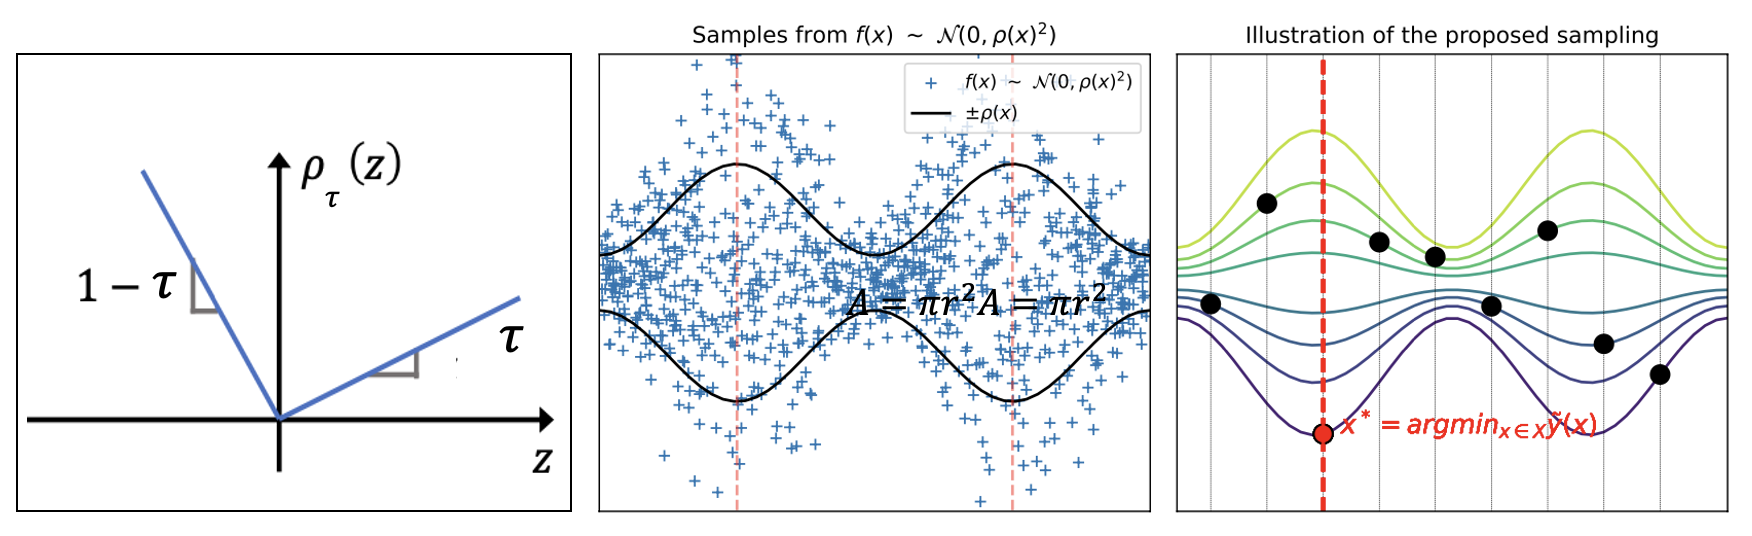
\includegraphics[scale=0.53]{figs/pinball_loss_and_CQR.png}
		\refstepcounter{figure}
   		\addcontentsline{lof}{figure}{Figure~\thefigure: Pinball loss and CQR within Bayesian optimization}
		\label{fig:CQR}
		\parbox{\linewidth}{
	 	\vspace{0.5em}
 	 	{\small \textit{Figure \ref{fig:CQR}:} Visualization of the Pinball loss function, where $z=y - \hat{y}$ (left) \cite{romano2019conformalized}; Samples from a synthetic heteroskedastic function (middle) and  the sampling procedure based on $|q| = 8$ predicted quantiles (right) \cite{salinas2023optimizing}.
 	 	}
 		}
	\end{figure}
	 
	 A close work is \cite{salinas2023optimizing} that employs \gls{cqr} to obtain quantiles with robust coverage during hyperparameter tuning via Bayesian optimization. Specifically, the calibrated quantiles are used to select the candidate for the next search, where a set of candidates is first sampled uniformly at random, and then for each of those candidates a random quantile is simply picked and is treated as the acquisition score (Figure \ref{fig:CQR}). We follow their notation and interpretation in defining the conformity score for a quantile surrogate:  
	 
	 \begin{equation}
		E_i = \max \big\{\hat{q}_{\tau_j}(x_i) - y_i, \; y_i - \hat{q}_{1-\tau_j}(x_i) \big\}
	 \vspace{0.7em}
	 \label{scoreCQR}
	 \end{equation}
	 
	 \noindent where $\hat{q}_{\tau}(x_i)$ denotes the predicted $\tau$-quantile at $x_i$. Note that the sign of the score is positive when the target $y_i$ is outside of the interval and negative when the target falls inside the predicted interval. This allows the conformity score to account for both overcoverage and undercoverage cases. In addition, the score amplitude always measures the distance to the closer quantile between $\hat{q}_{\tau_j}(x_i)$ and $\hat{q}_{1-\tau_j}(x_i)$ \cite{romano2019conformalized, salinas2023optimizing}.	 

\end{description}


\subsection{Conformal Prediction with Cross-validation}}
Solving a NAS problem is usually computationally expensive, as each neural architecture evaluation incurs the cost of fully training and validating the underlying model on the target dataset. Motivated by the fact that \gls{nas} based on Bayesian optimization is typically allocated with a budget of 100 to 200 epochs, an additional heuristic for constructing the calibration set via cross-validation (hereafter: \gls{cvcp}) is employed to avoid reducing the sample size for obtaining a holdout set as performed in \gls{scp}.

The \gls{cvcp} method is a natural extension of \gls{scp} and is first formally presented in  \cite{vovk2015cross}. At each step, the evaluated architectures are devided at random into $K$ folds. A dedicated surrogate model is trained on $K-1$ folds, while the remaining one is used as the calibration set to calculate the conformity scores. This process is repeated for $K$ times over each individual fold. Finally, conformity scores from all calibration folds are combined to form the overall calibration set, on which the quantile is computed to determine the calibration offset. For an unseen data point, the prediction is obtained by aggregating the predictions of the $K$ trained models, e.g., by taking the average of the model outputs.  Algorithm \ref{alg:CVCP} summarizes this procedure. 

\vspace{1em}
\begin{algorithm}[t]
  \caption{Conformal Prediction with Cross-validation}
  \label{alg:CVCP}
  \begin{algorithmic}[1]
    \textbf{Input:} 
    A set of observations $\{(x_{i}, y_{i})\}_{i=1}^n$, number of folds $K$, a prediction algorithm $h(\cdot)$, a non-conformity measure $\myfunc{s(\cdot)}$, nominal mis-coverage rate $\tau$, test data $x_{n+1}$. \vskip
    \textbf{Output:} a prediction set $\mathcal{C}_{\tau}(x_{n+1})}$ that covers $y_{n+1}$ with probability $1-\tau$. \vskip
    \vspace{0.5em}
    \STATE Initialise a conformity scoring set $S=\emptyset$
    \STATE Split the observations $\{(x_{i}, y_{i})\}_{i=1}^n$ into $K$ folds at random. $I_k$ denotes the index set containing indices of samples in the $k$-th fold.
    \FOR {$k$ in 1, 2, ..., K}
		\begin{enumerate}
    		\item Train $\hat{h}_{-k}(\cdot)$ on $\{(x_{i}, y_{i}) \mid i \notin I_k\}$
    		\item Compute conformity score on the $k$-th fold $S_k=\{s((\hat{h}_{-k}(x_{i}), y_i) \mid i \in I_k\}$
    		\item $S \leftarrow{S \cup S_k}$
    	\end{enumerate}
   	\ENDFOR
	\STATE Predict $x_{n+1}$: $h(x_{n+1}) \leftarrow aggregate(\{\hat{h}_{-1}(x_{n+1}), ..., \hat{h}_{-K}(x_{n+1})\})$ 
	\STATE Return $\mathcal{C}_{\tau}(x_{n+1}) \leftarrow \{y \,|\, s((h(x_{n+1}), y) \leq q\}$, where $q$ is the $\lceil(1-\tau)(n_s+1)\rceil$-th smallest value of $S$, with $n_s = |S|$.
    \end{algorithmic}
\end{algorithm}

Note that the only distinction between \gls{scp} and \gls{cvcp} is how the calibration set is constructed. Since it does not place any additional restriction on the choices of the underlying surrogate, \gls{cvcp} can be applied in conjunction with either ensemble predictor or quantile regressor in the same way as \gls{scp}. See Section \ref{sec:scp} for detailed configurations.

\subsection{Conformal Prediction with Bootstrapping}
Inspired by the fact that \gls{bananas} is built on an ensemble surrogate, we further explore incorporating Jackknife+-after-boostrap \cite{kim2020predictive}, a wrapper for predictive inference designed specifically for use with ensemble learners, into the calibration step (hereafter: \gls{btcp}).

In contrast to fitting $m$ neural networks on the same training data with different random weights initializations, as applied in the \gls{bananas} framework, a different technique to build an ensemble model is via bootstrapping. Specifically, the ensemble method starts by creating multiple training datasets by resampling the available data points with replacement. In the next step, multiple models are trained on each of the bootstrapped subsets, and their predictions are aggregated to produce the single final prediction \cite{breiman96}. This technique offers more accurate and stable estimates than a single model and has shown superior performance in application.

\begin{algorithm}[t]
  \caption{Conformal Prediction with Bootstrapping}
  \label{alg:BtCP}
  \begin{algorithmic}[1]
    \textbf{Input:} 
    A set of observations $\{(x_{i}, y_{i})\}_{i=1}^n$, number of bootstraps $B$, a prediction algorithm $h(\cdot)$, a non-conformity measure $\myfunc{s(\cdot)}$, nominal mis-coverage rate $\tau$, test data $x_{n+1}$. \vskip
    \textbf{Output:} a prediction set $\mathcal{C}_{\tau}(x_{n+1})}$ that covers $y_{n+1}$ with probability $1-\tau$. \vskip
    \vspace{0.5em}
    \STATE Sample all available data with replacement and create $B$ subsets. $I_b$ denotes the indices of data points included in the $b$-th sample.
    \STATE Train $\hat{h}_{b}(\cdot)$ on $\{(x_{i}, y_{i}) \mid i \in I_b\}$ for $b$ in 1, 2, ..., B
    \STATE Initialise a conformity scoring set $S=\emptyset$
    \FOR {$i$ in 1, 2, ..., n}
    	\begin{enumerate}
    		\STATE Initialize an empty for leave-one-out estimates $LOO_i=\emptyset$
    		\STATE For {$b$ in 1, 2, ..., B},  if {$i$ \notin \; $I_b$}\;: $LOO_i \leftarrow{LOO_i \cup \hat{h}_b(x_i)}$ 
			\STATE S \gets S \cup s\big(aggregate(LOO_i),\; y_i\big)
		\end{enumerate}
    \ENDFOR
	\STATE Predict $x_{n+1}$: $h(x_{n+1}) \leftarrow aggregate(\{\hat{h}_{1}(x_{n+1}), ..., \hat{h}_{B}(x_{n+1})\})$ 
	\STATE Return $\mathcal{C}_{\tau}(x_{n+1}) \leftarrow \{y \,|\, s((h(x_{n+1}), y) \leq q\}$, where $q$ is the $\lceil(1-\tau)(n_s+1)\rceil$-th smallest value of $S$, with $n_s = |S|$.
    \end{algorithmic}
\end{algorithm}

Jackknife+ is a type of \gls{cp} algorithm that is closely related to the \gls{loo} method \cite{barber2020jackknife}. Given a set of observations $\{(x_{i}, y_{i})\}_{i=1}^n$, the idea is to fit an \gls{loo} estimator $\hat{h}_{-i}$ using all available data except for the $i$-th sample, and this process iterates over all individual samples. Then, the predictive interval around the $i$-th point is obtained by offsetting the prediction from $\hat{h}_{-i}(x_i)$ with the quantile of all \gls{loo} conformity scores.  Equivalently, Jackknife+ can be viewed as a special case of \gls{cvcp} when the number of folds is exactly set to $K=n$.

Jackknife+-after-boostrap \cite{kim2020predictive} integrates both approaches and provides a cost-efficient wrapper by leveraging only the available bootstrapped sets and their corresponding fitted models, thereby avoiding re-fitting ensembles on each individual bootstrapped sample. \cite{pmlr-v139-xu21h} extends this method to online setting and proves its efficiency for time-series data. In contrast to the \gls{cp} algorithms described in earlier sections, \gls{btcp} requires no data splitting because sampling with replacement automatically creates holdout sets. Training the bootstrap ensemble on random subsets from the full data also reduces the chance of overfitting.

Implementation of \gls{btcp} is shown in Algorithm \ref{alg:BtCP}. Noteably, if a particular  data point appears in all bootstrapped samples, it is then excluded from the computation of conformity scores since it has no associated \gls{loo} estimator. In \gls{btcp}, the absolute residual is mainly used for measuring conformity, due to potentially insufficient \gls{loo} outputs for standard deviation estimation, i.e., $LOO_i$ in Algorithm \ref{alg:BtCP} might have fewer than two points. Specifically, \gls{btcp} is only applied with the ensemble model. This concludes our experiment setups and the \gls{bananascp} framework is finally evaluated under five various predictor+CP configurations.


\section{Distribution Estimation}
\label{sec:distest}
As described in Section \ref{sec:bananas}, Bayesian optimization generally relies on a continuous posterior distribution at $X=x$ to obtain the acquisition score. In this section, we discuss how the conditional distribution is estimated and evaluated. Here, we denote by $F_t(x)$ the \gls{cdf} of the posterior distribution of the data point $x$ at step $t$. In the context of NAS, where the target variable is assumed to be continuous and real-valued, the distribution can be represented by the inverse of its \gls{cdf}, or quantile function without loss of generality, i.e. $Q_{t}(x) = F^{-1}_{t}(x)$. 

\vspace{0.3em}
In the \gls{bananascp} framework, as outlined in Algorithm \ref{alg:OCP}, we are able to generate calibrated quantile estimates for a finite set of discrete quantile levels. Intuitively, assuming the quantiles estimates are accurate, increasing the granularity of quantile levels should lead to a more accurate approximation of the underlying continuous distribution. However, it is computationally prohibited to estimate an infinite number of quantiles in practice, especially with significantly limited training data. Therefore, we propose an approach for constructing a continuous distribution from discrete quantile estimates with mild assumption. Specifically, the distribution estimator is defined as:

\begin{description}[leftmargin=0cm, listparindent=\parindent]
\item[Definition] Let $\{q_i\}_{i=1}^n$ be a quantile of percentile levels such that $0<q_1<q_2, ..., <q_n<1$, and $\{v_i\}_{i=1}^n$ are the corresponding quantiles, i.e., $F^{-1}(q_i)=v_i$, the empirical \gls{cdf} of the distributions $\hat{F}$ is constructed by applying linear interpolation between adjacent quantiles. Consequently, the \gls{pdf} of a specific interval $\left(v_a, v_b\right), a,b \in \{1,..., n\}$ and $a<b$ is:
\vspace{0.5em}
\[
PDF(x) = \frac{q_b - q_a}{v_b - v_a}, \quad & \text{if } x \in (v_a, v_b) \\
\]

\vspace{1em}
\item[Diagnosis Analysis] To assess the validity of this approach, we first perform a diagnosis analysis using synthetic datasets generated by a left-skewed Gaussian distribution, which we believe resembles the true underlying distribution of the validation performances of architectures in a search space. The experiments on the synthetic data are intended to reflect the comparisons in a real \gls{nas} application, therefore two kinds of distribution estimators are examined: a Gaussian estimator and a linear-interpolation based quantile estimator. The analysis is repeated with different parameterizations, e.g, the number of quantiles, or the size of the samples, etc.

Table \ref{table:distest} reports the performance of three distribution estimators on synthetic datasets with various sample sizes. In particular, the linear-interpolation based quantile estimator is evaluated under 10 and 20 quantile levels, and the quantile estimates for interpolation are obtained by taking the empirical quantiles of the sample data. The estimation performance is assessed using the mean, standard deviation and Kullback–Leibler (KL) divergence \cite{kullback1951information}. For each sample size, we run 50 trials and aggregate the metrics over the trials to reduce the effects of randomness. Results in Table \ref{table:distest} indicate that the linear-interpolation based quantile estimator offers a better approximation to an asymmetric distribution than a Normal distribution, and increasing the number of quantile levels leads to improved approximation performance, provided with sufficient data. However, a caveat is that quantile-based estimation tends to produce biased standard deviation estimates, which may lead to undesired effect.

Having considered the behaviors of the various acquisition functions employed in the real \gls{bananascp} application (see Section \ref{sec:acq}), we additionally present several visualizations based on a synthetic dataset with 150 samples (Figure \ref{fig:distest10}, Figure \ref{fig:distest20}) to confirm the shapes of the estimated distributions are not significantly deviated from that of the true underlying distribution, thereby assuring the effectiveness of the acquisition functions.

\vspace{0.5em}
\item[Evaluation Metrics] Within the \gls{bananascp} framework, the calibration quality at a specific epoch is measured by the \gls{rmsce} \cite{pmlr-v80-kuleshov18a}. Suppose $\hat{F}^{-1}_t$ is the \gls{cdf} of the distribution estimated at the  $t$-th step and $y_t$ is the true value revealed after the estimation, consider a sequence of $\{(\hat{F}^{-1}_t, y_t)\}_{t=1}^T$ that represents a neural architecture search process after $T$ epochs, the calibration error at the $T$-th epoch is defined as:
	\vspace{0.5em}
	\begin{equation}
	\text{RMSCE} \left( \hat{F}^{-1}_1, y_1, \dots, \hat{F}^{-1}_T, y_T \right) = \sum_{j=1}^m w_j \left( p_j - \hat{p}_j \right)^2
	\label{rmsce}
	\end{equation}

	\[
	\text{with} \quad
	\hat{p}_j = \frac{\left| \left\{ y_t \;\middle|\; \hat{F}^{-1}_t(y_t) \le p_j,\; t = 1, 2, \dots, T \right\} \right|}{T}
	\]

\noindent where $m$ represents the number of discrete quantile levels and the scalars $w_j$ are  quantile weights. For simplicity, we adopt  $w_j=1, \forall j \in[0,1]$ in this work. Alternatively, calibration errors of the quantiles can be weighted by the number of observations falling into the corresponding intervals. Note that calibration errors calculated with different numbers of quantiles are not directly comparable. In general, increasing the number of quantiles tends to lead to larger calibration errors.	
\end{description}


\begin{table}[htbp]
\centering
\refstepcounter{table}
\addcontentsline{lot}{table}{Table~\thetable: Statistical Comparison of Distribution Estimators}

\parbox{\linewidth}{
  {\small \textit{Table \ref{table:distest}}: Statistical metrics of distributions estimated by three methods on synthetic datasets with sample size ranging from 50 to 500. For each method and sample size, the mean, standard deviation, and KL divergence are reported to assess the estimation performance.}  
}

\label{table:distest}
\vspace{2em}
\begin{tabular}{llc>{\centering\arraybackslash}p{2.5cm}c}
\toprule
\textbf{Sample Size} & \textbf{Estimator} & \textbf{Mean} & \textbf{Standard Deviation} & \textbf{KL Divergence} \\
\midrule
\multirow{50}  & Gaussian            & -0.7985 & 0.6005 & 0.5727 \\
               & Quantile ($|q|=10$) & -0.7481 & 0.5503 & 0.1646 \\
               & Quantile ($|q|=20$) & -0.7440 & 0.5536 & 0.2928 \\
\midrule
\multirow{100} & Gaussian            & -0.7989 & 0.6145 & 0.6181 \\
               & Quantile ($|q|=10$) & -0.7744 & 0.5941 & 0.0953 \\
               & Quantile ($|q|=20$) & -0.7654 & 0.5798 & 0.1297 \\       
\midrule
\multirow{150} & Gaussian            & -0.7986 & 0.6100 & 0.5977 \\
               & Quantile ($|q|=10$) & -0.7860 & 0.6133 & 0.0811 \\
               & Quantile ($|q|=20$) & -0.7791 & 0.5950 & 0.0948 \\
\midrule    
\multirow{200} & Gaussian            & -0.7969 & 0.6162 & 0.6227 \\
               & Quantile ($|q|=10$) & -0.7948 & 0.6347 & 0.0625 \\
               & Quantile ($|q|=20$) & -0.7833 & 0.6050 & 0.0676 \\
\midrule   
\multirow{250} & Gaussian            & -0.7921 & 0.6127 & 0.6166 \\
               & Quantile ($|q|=10$)	 & -0.7936 & 0.6384 & 0.0526 \\
			   & Quantile ($|q|=20$) & -0.7815 & 0.6084	& 0.0576 \\
\midrule 
\multirow{300} & Gaussian            & -0.7940 & 0.6140 & 0.6168 \\
               & Quantile ($|q|=10$)	 & -0.8002 & 0.6521 & 0.0540 \\
               & Quantile ($|q|=20$)	 & -0.7876 & 0.6153	& 0.0482 \\
\midrule 
\multirow{350} & Gaussian            & -0.7919 & 0.6131 & 0.6176 \\
               & Quantile ($|q|=10$)	 & -0.8002 & 0.6570 & 0.0507 \\
               & Quantile ($|q|=20$)	 & -0.7866 & 0.6188	& 0.0432 \\
\midrule      
\multirow{400} & Gaussian            & -0.7919 & 0.6131 & 0.6174 \\
               & Quantile ($|q|=10$) & -0.8041 & 0.6650 & 0.0491 \\
               & Quantile ($|q|=20$)	 & -0.7871 & 0.6215	& 0.0388 \\
\midrule 
\multirow{450} & Gaussian            & -0.7908 & 0.6114 & 0.6121 \\
               & Quantile ($|q|=10$) & -0.8054 & 0.6668 & 0.0468 \\
               & Quantile ($|q|=20$) & -0.7888 & 0.6240	& 0.0357 \\
\midrule 
\multirow{500} & Gaussian            & -0.7922 & 0.6081 & 0.5956 \\
               & Quantile ($|q|=10$) & -0.8070 & 0.6657 & 0.0459 \\
               & Quantile ($|q|=20$) & -0.7912 & 0.6219	& 0.0328 \\
\midrule
-&Ground Truth & -0.7939 & 0.6080 & 0.0000 \\
\bottomrule
\end{tabular}
\end{table}

\begin{landscape}
% First Row (10 Quantiles)
\begin{figure}[H]
  \refstepcounter{figure}
  \addcontentsline{lof}{figure}{Figure~\thefigure: Visualization of Estimated Distribution Based on 10 Quantiles.} 
  \label{fig:distest10}
  \centering
  \begin{minipage}[b]{0.4\textwidth}
    \centering
    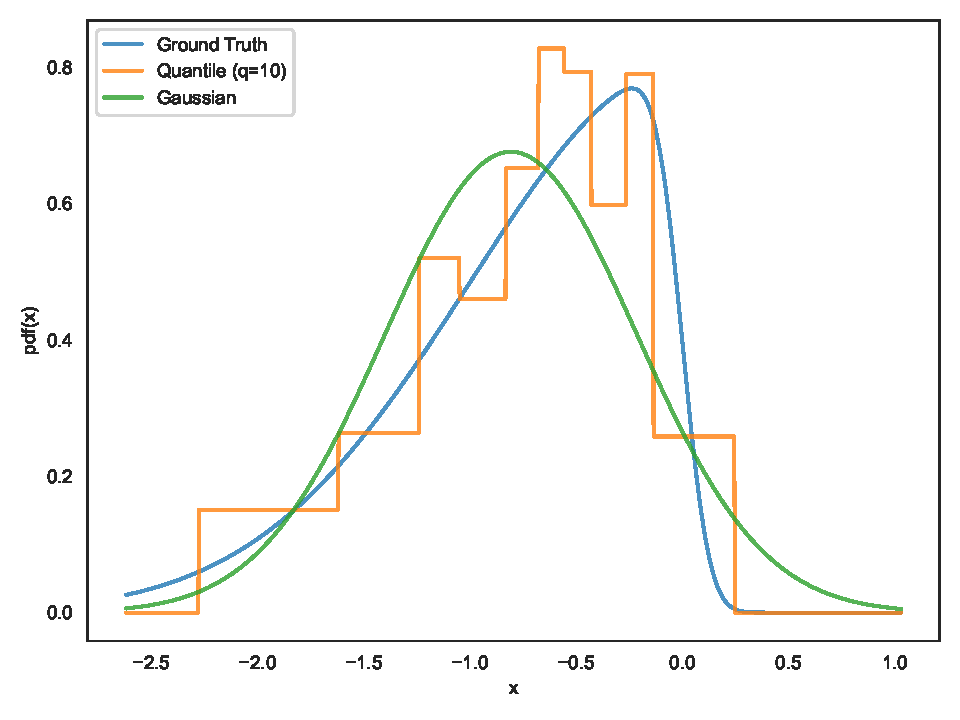
\includegraphics[width=\linewidth]{figs/10_pdf_plot.pdf}
    \\[0.5em]
    {\small (a)}
  \end{minipage}
  \hfill
  \begin{minipage}[b]{0.4\textwidth}
    \centering
    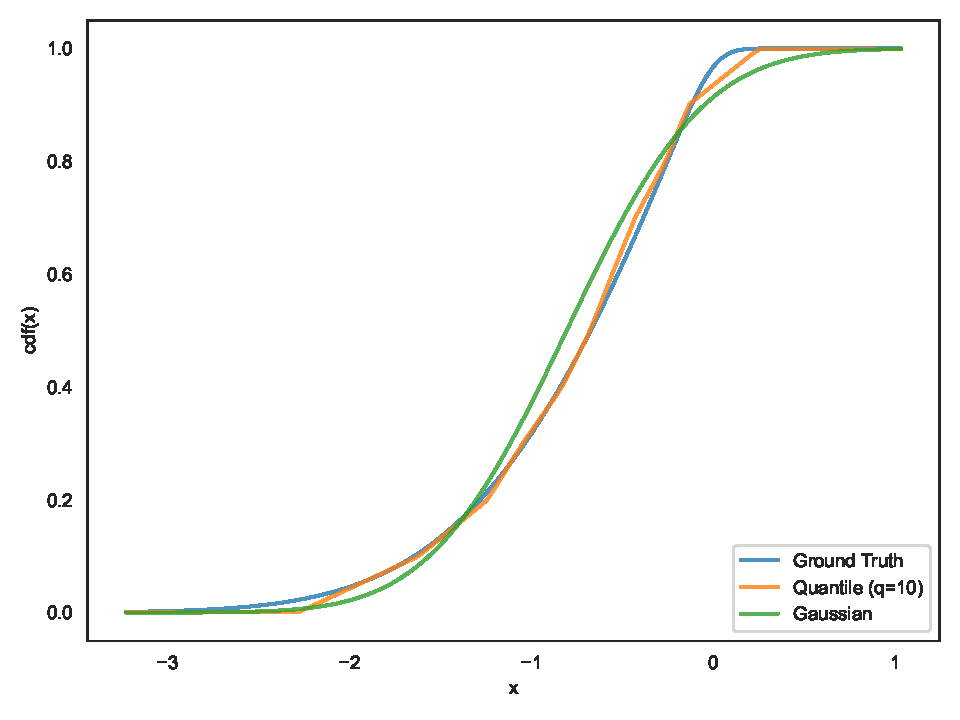
\includegraphics[width=\linewidth]{figs/10_cdf_plot.pdf}
    \\[0.5em]
    {\small (b)}
  \end{minipage}
  \hfill
   \begin{minipage}[b]{0.4\textwidth}
    \centering
    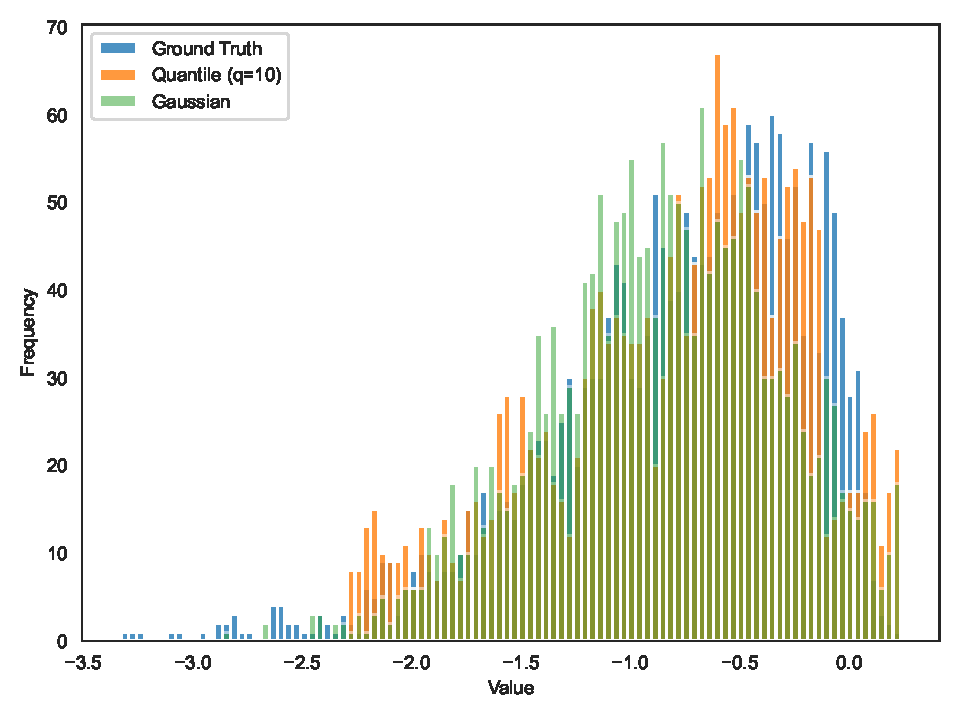
\includegraphics[width=\linewidth]{figs/10_rvs_plot.pdf}
    \\[0.5em]
    {\small (c)}
  \end{minipage}
 
 \vspace{1em}
 \parbox{\linewidth}{
 	 {\small \textit{Figure \ref{fig:distest10}:} Visualization of the distributions estimated from 10 quantile levels using a synthetic dataset with 150 samples. The figure includes the estimated \gls{pdf} (a), \gls{cdf} (b), and the histogram of 2000 samples drawn from the estimated distribution (c).}
 }
\end{figure}

% Second Row (20 Quantiles)
\begin{figure}[H]
  \refstepcounter{figure}
  \addcontentsline{lof}{figure}{Figure~\thefigure: Visualization of Estimated Distribution Based on 20 Quantiles.} 
  \label{fig:distest20}
  \centering
  \begin{minipage}[b]{0.4\textwidth}
    \centering
    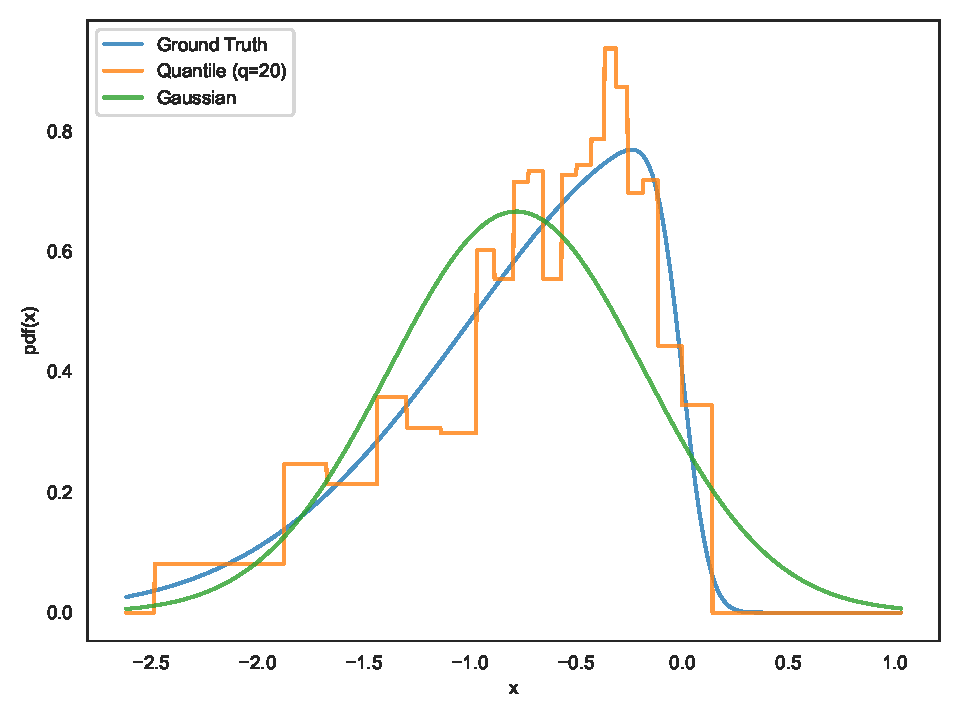
\includegraphics[width=\linewidth]{figs/20_pdf_plot.pdf}
    {\small (a)}
  \end{minipage}
  \hfill
  \begin{minipage}[b]{0.4\textwidth}
    \centering
    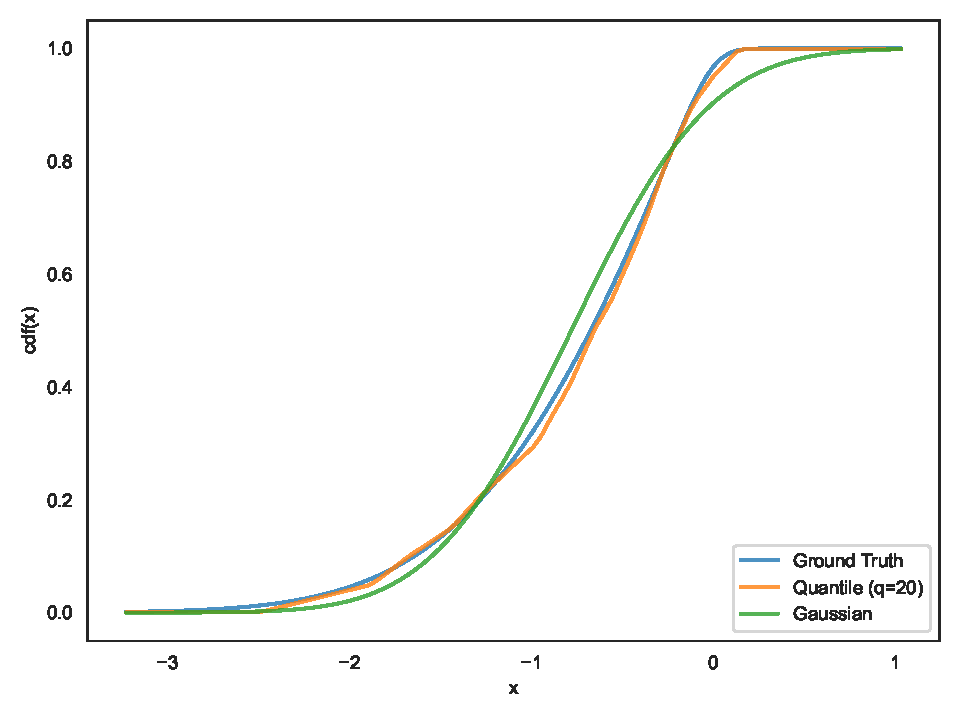
\includegraphics[width=\linewidth]{figs/20_cdf_plot.pdf}
    \\[0.5em]
    {\small (b)}
  \end{minipage}
  \hfill
   \begin{minipage}[b]{0.4\textwidth}
    \centering
    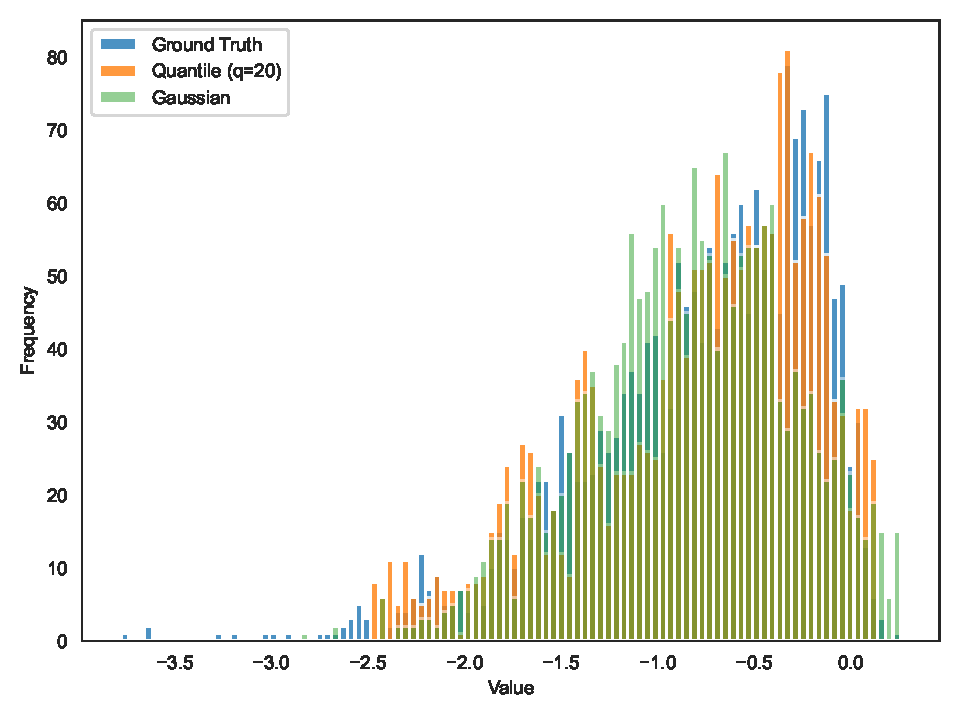
\includegraphics[width=\linewidth]{figs/20_rvs_plot.pdf}
    \\[0.5em]
    {\small (c)}
  \end{minipage}
  \vspace{1em}
  
 \parbox{\linewidth}{
 	 {\small \textit{Figure \ref{fig:distest20}:} Visualization of the distributions estimated from 20 quantile levels using a synthetic dataset with 150 samples. The figure includes the estimated \gls{pdf} (a), \gls{cdf} (b), and the histogram of 2000 samples drawn from the estimated distribution (c).}
 }
\end{figure}
\end{landscape}

\vspace{1em}
\section{Acquisition Function and Search Strategy}
\label{sec:acq}
Finally, we describe the acquisition functions and the aquisition optimization strategies used within the \gls{bananascp} framework.

\vspace{0.1em}
\subsection{Acquisition Function}
\label{subsec:acq_func}
We consider four commonly used acquisition functions. Consistent with the notation in the previous sections, $\hat{f}(a)$ is the predicted performance of architecture $a$ and $\hat{F}_a$ represents the \gls{cdf} of the estimated distribution of $f(a)$. Then, depending on the acquisition function used, the specific acquisition score can be calculated by: 

\begin{description}[leftmargin=0cm, itemsep=1pt] 
\item[\gls{its}:] A sample is drawn from the distribution at random and its value is seen as the acquistion score for the candidate architecture $a$.
\item[\gls{ucb}:] The acquisition score is given by $\mu+\gamma \cdot \sigma$ for a Gaussian distribution, where $\gamma$ is the exploration factor. For non-Gaussian distributions, we follow \cite{deshpande2024online} and generalize the function to a quantile function, i.e., $\hat{F}^{-1}_a(\gamma)$.  As in the original formulation, higher values of $\gamma$ promotes exploration. In our experiments, we set $\gamma=0.75$ due to these concerns: a) the distribution of model performance is believed to be left-skewed; b) estimates of extreme quantiles are generally based on sparse observations and therefore might be less reliable. A value of 0.75 is likely to offer a reasonable trade-off between exploration and accurate estimation.
\item[\gls{pi}:] The probability of improvements corresponds to $1 - \hat{F}^{-1}_a(f_{max})$, with $f_{max}$ being the highest model performance ever observed.
\item[\gls{ei}:] The expected value of improvements can be written as $\mathbb{E}[\max(0,  f(a)- f_{max}})]$, with $f_{max}$ being the highest model performance ever observed. 
\end{description}

\vspace{0.1em}
\subsection{Acquisition Optimization Strategy}
\label{subsec:acq_strats}
In parallel to the settings in \cite{white2019bananas} (see Section \ref{sec:bananas}), we compare three different approaches for constructing a set with 100 \footnote{ We have conducted preliminary experiments using 1,000 candidate samples. The results indicate that increasing the sample size does not lead to significant improvements in performance. Considering the size of the search space (NAS-Bench-201), and the required computational time, the candidate set size is fixed at 100 for all subsequent primary experiments.} candidates in order to compute the acquisition scores. The motivations and the  specific approaches are described below:
 
\begin{description}[leftmargin=0cm, itemsep=1pt]
\item[Mutation] We investigate the mutation-based search strategy because this approach demonstrates the best performance in \cite{white2019bananas}. In line with their approach, the candidates are selected by randomly changing one operation or one edge of the $k$ best models that have been found so far, where $k$ is a search hyperparameter with the default value of 2. 
\item[Random Sampling] This approach is explored under the assumption that globally sampled architectures may improve the quality of the calibration process. As indicated by the name, the candidate set is created by randomly sampling architectures from the entire search space.
\item[Dynamic] This approach aims to resemble the "random + mutation" search strategy in \cite{white2019bananas}. The search process begins with random sampling until utilizing the first half of the search budget, then switches to a mutation-based strategy that progressively reduces the number of best ever-found models considered for mutation. To be precise, the number of models to be mutated decreases by 2 every 20 epoch. For instance, in a \gls{nas} task with 160 epochs, candidates are picked via random sampling for the first 80 epochs. Starting from epochs 80/100/120/140, the candidates are selected by mutating the best 8/6/4/2 models, respectively.
\end{description} 



% chapter 4
\chapter{Experiment Design}
\label{ch4}
To compare the performance of BANANAS--CP with the original BANANAS method and assess the role of uncertainty calibration, we choose the widely used tabular benchmark dataset NAS-Bench-201 \cite{dong2020nasbench201} for experiments. In this chapter, we first provide a description of the dataset (Section \ref{sec: dataset}). Then, we introduce the general setups that are shared across all experiments, along with the strategy for step-wise configuration tuning  (Section \ref{sec: setups}).

\section{Dataset}
\label{sec: dataset}
NAS-Bench-201 is a cell-based architecture search space. Each cell is expressed as a densely connected \gls{dag} with in total 4 nodes and 6 edges. The nodes within a cell represents the sum of all feature maps transformed through the associated operations of the edges pointing to this node, and the edges represent the architectures operation that are chosen from the predefined operation set. Specifically, the operation set comprises 5 representative operations: (1) zeroize, (2) skip connection, (3) 1-by-1 convolution, (4) 3-by-3 convolution, and (5) 3-by-3 average pooling layer. This search space contains all possible architectures generated by 4 nodes and 5 associated operation options, which results in 15,625 cell candidates in total. The macro structure of an architecture is defined as a chain of blocks, which is initiated with one 3-by-3 convolution with 16 output channels and a batch normalization layer, and consists of three stacks of cells that are connected by a residual layer. Figure \ref{fig: nasbench201} illustartes the structure of an architecture in this search space.  
	\vspace{0.5em}	
	\begin{figure}[bthp]
		\centering
		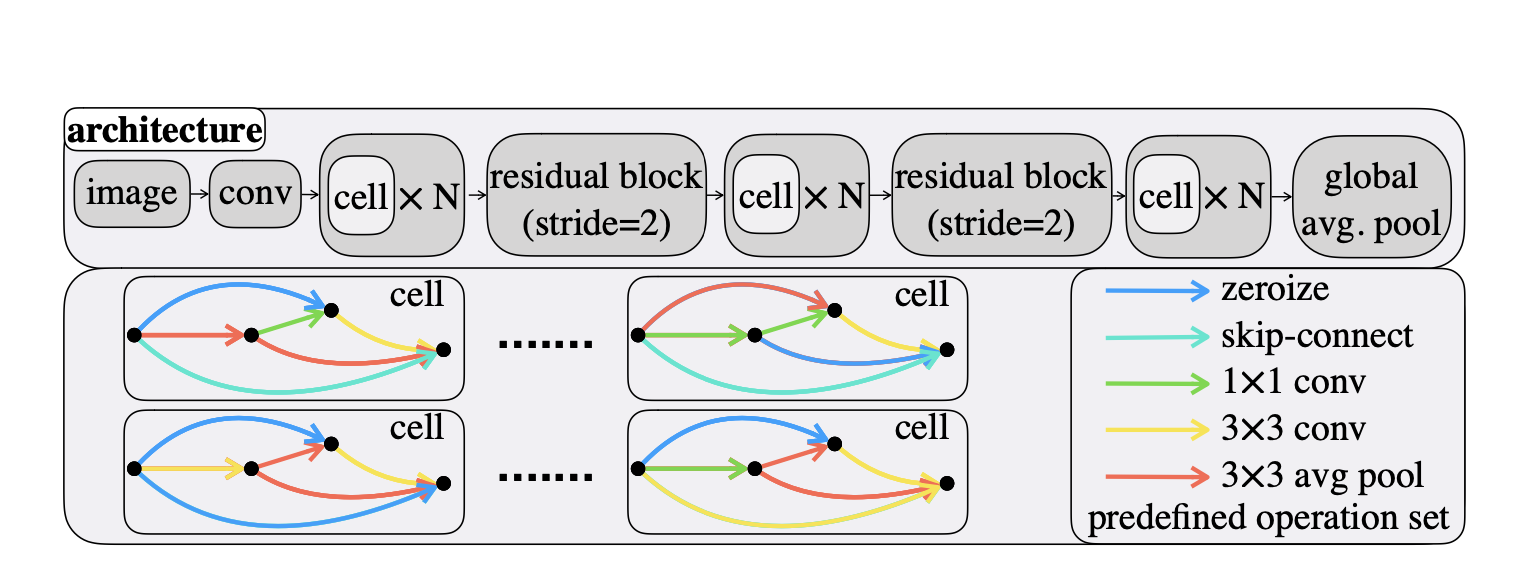
\includegraphics[scale=0.48]{figs/nas_bench_201.png}
		\refstepcounter{figure}
   		\addcontentsline{lof}{figure}{Figure~\thefigure: Illustration of the overall network architecture structure in NAS-Bench-201}
		\label{fig: nasbench201}
			\parbox{\linewidth}{
	 		\vspace{0.7em}
 	 		{\small \textit{Figure \ref{fig: nasbench201}:} Illustration of the skeleton (top) and the design of individual cells (bottom) of architectures in NAS-Bench-201 \cite{dong2020nasbench201}.
 	 		}
 		}
	\end{figure}
\newline

\newline
Architectures in the search space are evaluated on three datasets that are widely used for image classification tasks: CIFAR-10, CIFAR-100 \cite{krizhevsky2009learning} and ImageNet-16-120 \cite{chrabaszcz2017downsampled}. Each dataset is split into the training, validation, and test sets using a standard evaluation pipeline. NAS-Bench-201 provides the training, validation, and test losses as well as accuracies for all architectures in the search space. The following gives a brief introduction to these datasets:

\begin{description}[leftmargin=0cm, listparindent=\parindent]
 	\item[CIFAR10]:	The dataset consists of 60K $32\times32$ color images in 10 classes. In NAS-Bench-201, 25K images with 10 classes are assigned into the training and the validation sets, respectively. The test set contains 10K images, with 1K images per class.
 	\item[CIFAR100]: This dataset has the same images as CIFAR-10 but in 100 classes. The training set has 50K images, and each of the validation and the test sets has 5K images.
 	\item[ImageNet-16-120]: This dataset contains 151.7K training images, 3K validation images, and 3K test images with 120 classes. Each image has 16$\times$16 pixels.
\end{description} 


Since its introduction, NAS-Bench-201 has contributed to the \gls{nas} community in several aspects. First, it provides full training and test results (e.g., accuracy, training time, etc.) for every possible architecture in the space on three datasets, allowing reproducible NAS experiments without training models from scratch. Because all architectures are pre-evaluated, \gls{nas} methods can be benchmarked extremely efficiently and subsequent \gls{nas} research can just focus on the search algorithms without any model evaluation. Moreover, using a unified dataset splitting strategy, NAS-Bench-201 reduces the variability caused by different implementation details or training setups, which is a limitation of previous benchmarks, and thus enables consistent comparisons across different \gls{nas} algorithms. 

\vspace{0.2em}	
NAS-Bench-201 also serves as a foundation for extending benchmark datasets. In particualr, \cite{jung2023neural} evaluates all 6,466 non-isomorphic architectures in the space for robustness against adversarial attacks and common image corruptions, and introduces a dataset that includes both clean and robust accuracy values. This dataset covers adversarial attacks and corruptions of different severity levels, enabling a systematical study on how architectural variations impact robustness.

\vspace{0.2em}
In this work, we leverage the API offered by NAS-Bench-201 and directly query the pre-computed train and test metrics of architectures \footnote{Performance metrics for training and testing on the three datasets are downloaded from NASLib: \ulr{https://github.com/automl/NASLib/tree/Develop}}. Notably, NAS-Bench-201 also provides several analytical metrics, such as model rankings and accuracy correlations across the three datasets, which further guide our post-hoc analysis of the experimental results.


\section{Setups and Implementation}
\label{sec: setups}
We now present the common experimental setups used throughout this study. As introduced in Chapter \ref{ch3}, we primarily run experiments for five calibrated NAS algorithms varying in calibration techniques and/or surrogate predictors: \gls{scp} with ensemble predictor, \gls{scp} with quantile regressor, \gls{cvcp} with ensemble predictor, \gls{cvcp} with quantile regressor, and \gls{btcp} with ensemble predictor. In line with \cite{white2019bananas}, each algorithm is given a search budget of 150 epochs to ensure consistent benchmarking with \gls{bananas}. As in previous works, the validation accuracy is used as the supervision signal to guide the search. Each algorithm is repeated for 50 trials with different random seeds and the final results are obtained by aggregating the performance across all trials. 

\vspace{0.2em}
Although training neural networks is avoided thanks to the benchmark datset, each search algorithm still involves a large number of hyperparameters, making it unrealistic to tune them all. Also, not all hyperparameters have the same impact on search performance; some might be more important than the others. Therefore, we select a subset of hyperparameters that we believe, either base on experience or preliminary testing results, are less important or already well-set, and fix their values throughout the experiments. For instance, we believe path-encoding is stronger than other architecture encoding techniques, thus architectures are always encoded using paths present in the cell in all experiments. As for the acquisition optimization strategy, the number of candidates that the acquisition function evaluates in each iteration is fixed at 100 and the maximal mutation allowed for each model is  1 in case the mutation strategy is adopted. In addition, we follow \cite{white2019bananas} and output 10 architectures to mimic the parallelized evaluation procedure.
\vspace{0.2em}

The hyperparameters are tuned progressively. In the first stage, we focus on configurations common to all algorithms. We start by conducting a thorough analysis on the baseline method, i.e., \gls{scp} with ensemble predictor, to find the optimal general setting, like the number of quantiles, the size of the initial dataset (the number of model evaluations before fitting the surrogate), the acquisition functions and the sampling strategies, etc. This optimal setting will be applied to other more advanced approaches in the next stage. Then, we turn to hyperparameter specific to each search algorithm and 
	conduct separate experiments that are  discussed in the respective sections.

\vspace{0.2em}
We borrow the implementation of \gls{bananas} from NASLib \footnote{https://github.com/automl/NASLib}, which is a modern Python-based framework for \gls{nas} developed by the AutoML Freiburg group. NASLib is well modularized, enabling a relatively easy integration of the new calibration block. In NASLib, each \gls{nas} algorithm typically comprises a \textit{trainer} for initiating search and evaluation iterations and an \textit{optimizer} for encapsulating specific search logics, including an inherent \textit{predictor} if applicable. Specifically, \textit{trainer} serves as a generic engine and is shared across all NAS algorithms. All predictors should conform to a particular interface so that they can be invoked inside the \textit{trainer}. 

\vspace{0.2em}
Building on this structure, we add new modules for constructing the \gls{bananascp} framework, including a quantile regressor, distribution estimators (along with the compatible acquisition functions), and the calibration algorithms. We leverage the existing implementation for \textit{trainer} with mild modifications on the export functionalities, aiming for a better access to intermediate outputs, such as the estimated distribution at each iteration. In addition, we also provide tools for analyzing and interpreting the experimental results.

% chapter 5
\chapter{Experiment Results}
This chapter presents the performance of the methods introduced in Chapter \ref{ch3}, evaluated using the experimental setups described in Chapter \ref{ch4}. 

\section{Baseline}
\label{sec: baseline}
We begin with the baseline strategy, \gls{scp} with the ensemble predictor. 



% chapter 6
\chapter{Conclusion}
This chapter presents the central findings of this work as well as their critical discussions (Section \ref{sec: discussion}). Finally, it highlights limitations and corresponding opportunities for further research (Section \ref{sec: future_work}).

\section{Discussion}
\label{sec: discussion}

\section{Limitations and Future Work}
\label{sec: future_work}


% Reference
\bibliographystyle{plain}
\bibliography{references}

% Appendix
% List of algorithms/figures/tables
\listofalgorithms 
\listoffigures 
\listoftables
\printglossary[type=\acronymtype, title=Acronyms]

\appendix
\chapter{Program Code and Data Resources}
The source code and a documentation are available at the GitHub repository: \url{https://github.com/chengc823/Thesis.}
The datasets used for experiments and algorithm evaluations are sourced from the \href{https://github.com/automl/NASLib/tree/Develop}{NASLib repository}.

In case of access or permission issues to the private repository, please reach out at: chechen@mail.uni-mannheim.de.

\chapter{Additional Experimental Results}


% Declare non-Plagiarism and independent work
\backmatter
\chapter{Ehrenwörtliche Erklärung}
Ich versichere, dass ich die beiliegende Bachelor-, Master-, Seminar-, oder
Projektarbeit ohne Hilfe Dritter und ohne Benutzung anderer als der angegebenen
Quellen und in der untenstehenden Tabelle angegebenen Hilfsmittel angefertigt
und die den benutzten Quellen wörtlich oder inhaltlich entnommenen Stellen als
solche kenntlich gemacht habe. Diese Arbeit hat in gleicher oder ähnlicher Form
noch keiner Prüfungsbehörde vorgelegen. Ich bin mir bewusst, dass eine falsche
Erklärung rechtliche Folgen haben wird.

% Declare the use of AI tools.
\vspace{0.5cm}
  \textbf{Declaration of Used AI Tools} \\[.3em]
  \begin{tabularx}{\textwidth}{lXlc}
    \toprule
    Tool & Purpose & Where? & Useful? \\
    \midrule
    ChatGPT & Rephrasing & Throughout & + \\
    ChatGPT & Debugging LaTeX syntax errors  & Equation & + \\
    ChatGPT & Rendering LaTeX tables from Python frame & Tables & + \\
    \bottomrule
  \end{tabularx}
\end{center}

\vspace{2cm}
\noindent Unterschrift\\
\noindent Mannheim, den 30.07.2025 \hfill

\end{document}
